\documentclass[a4paper,12pt]{article}
\usepackage{path}
\usepackage[spanish]{babel}
\usepackage{graphicx}
\graphicspath{{../img/}}
\usepackage[section]{placeins}
\usepackage{hyperref}
\hypersetup{
    colorlinks = true,
    linkcolor = blue,
    urlcolor = cyan
}
\usepackage[T1]{fontenc}
\usepackage{graphicx}
\usepackage{xcolor}
\usepackage{float}
\usepackage{enumitem}
\usepackage{booktabs}
\usepackage{geometry}
\usepackage{titlesec}
\usepackage{fancyhdr}
\usepackage{parskip}
\usepackage{microtype}
\usepackage{pmboxdraw}

\geometry{margin=2.5cm}
\setlength{\parskip}{1em}
\setlength{\parindent}{0pt}

\definecolor{myblue}{HTML}{005F9E}
\definecolor{mygray}{HTML}{4D4D4D}
\definecolor{mycyan}{HTML}{008B8B}


\usepackage{lmodern}
\renewcommand{\familydefault}{\sfdefault}

\titleformat{\section}
  {\Large\bfseries\color{myblue}}
  {\thesection}{1em}{}

\titleformat{\subsection}
  {\large\bfseries\color{myblue}}
  {\thesubsection}{1em}{}

\titleformat{\subsubsection}
  {\normalsize\bfseries\color{mygray}}
  {\thesubsubsection}{1em}{}

\pagestyle{fancy}
\fancyhf{}
\fancyhead[L]{\textit{Sistemas de Gestión Empresarial}}
\fancyhead[R]{\thepage}
\renewcommand{\headrulewidth}{0.4pt}
\renewcommand{\headrule}{\hbox to\headwidth{\color{myblue}\leaders\hrule height \headrulewidth\hfill}}

\title{
    \vspace{2cm}
    {\Huge\textbf{Sistemas de Gestión Empresarial}}\\[1em]
    {\Large\textbf{Práctica 2}}\\[1em]
    {\Large Implantación de Odoo como ERP para un negocio de venta de material de papelería}
    \vspace{1.5cm}
}

\author{\Large Daniel Calvar Cruz\\[0.5em]\normalsize 2º CS DAM}
\date{\vspace{1cm}\today}


\begin{document}

\maketitle
\clearpage
\hypertarget{anchor-indice}{}
\tableofcontents
\newpage

\section{Introducción}
\hyperlink{anchor-indice}{\textbf{Volver}}\\

Objetivo:

Los alumnos deberán implantar y configurar los módulos de Odoo indicados,
demostrar su funcionamiento mediante capturas de pantalla y explicar su utilidad.
Además, realizarán una copia de seguridad de la base de datos y del archivo de
configuración de Odoo (odoo.conf) mediante consola, documentando el proceso con
capturas.


\section{Módulos a instalar}
\hyperlink{anchor-indice}{\textbf{Volver}}\\

La práctica requiere del uso de los siguientes modulos: 
\begin{enumerate}
    \item Facturación
    \item Empleados
    \item Compras
    \item Ventas
    \item Punto de Venta
    \item Contactos
    \item CRM
\end{enumerate}

He escogido Contactos y CRM porque me han parecido de gran utilidad para ayudar al establecimiento de una buena estrategia de mercado, viable y escalable.

\begin{figure}[h!]
    \centering
    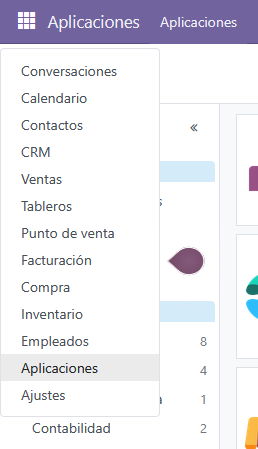
\includegraphics[width=0.5\textwidth]{pr2odoo01-modulosInstalados.png}
    \caption{Modulos instalados}
\end{figure}
\FloatBarrier

\clearpage

\section{Análisis de módulos}
\hyperlink{anchor-indice}{\textbf{Volver}}\\

Estos módulos forman parte del conjunto completo de herramientas empresariales de Odoo, cada uno especializado en un aspecto diferente de la gestión empresarial.

\subsection{Facturación}

El módulo de Facturación es fundamental para la gestión financiera de cualquier empresa. Este permite automatizar completamente el proceso de facturación, desde la generación de facturas hasta el seguimiento de pagos y estados de cuenta.

Una de sus principales ventajas es la capacidad de mantener un registro preciso y organizado de todas las transacciones financieras, facilitando así la elaboración de informes y el cumplimiento de obligaciones fiscales.

Además, se integra perfectamente con otros módulos como Ventas y Compras, permitiendo un flujo de información financiera sin obstrucciones a través de toda la empresa.

\begin{figure}[h!]
    \centering
    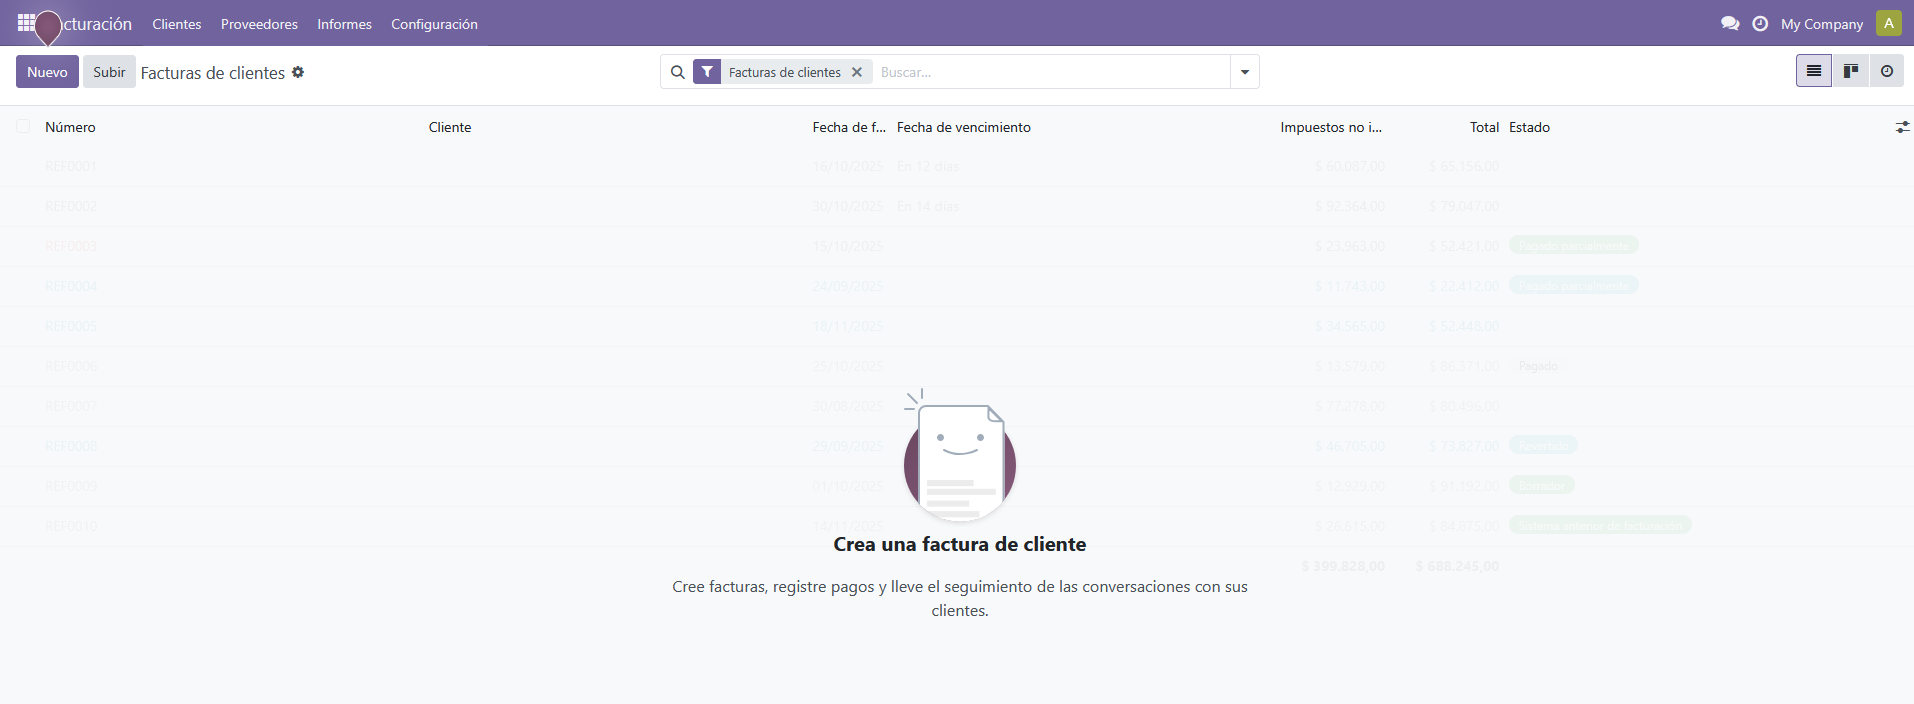
\includegraphics[width=1\textwidth]{pr2odoo02-facturacMain.png}
    \caption{Pantalla principal de Facturación}
\end{figure}
\FloatBarrier

\clearpage

Rellenamos los campos con la información pertinente.

\begin{figure}[h!]
    \centering
    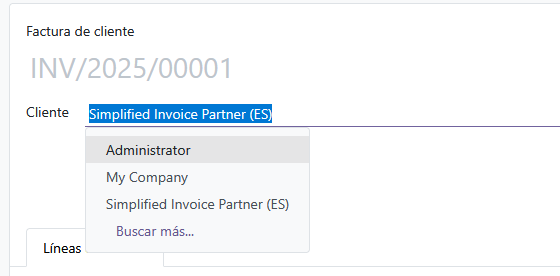
\includegraphics[width=0.8\textwidth]{pr2odoo03-facturac01.png}
    \caption{Cliente}
\end{figure}
\FloatBarrier

\begin{figure}[h!]
    \centering
    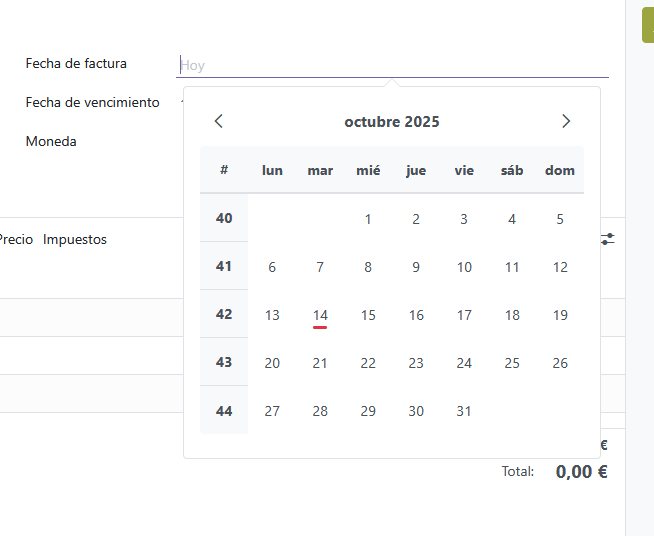
\includegraphics[width=0.8\textwidth]{pr2odoo04-facturac02.png}
    \caption{Fechas de factura}
\end{figure}
\FloatBarrier

\begin{figure}[h!]
    \centering
    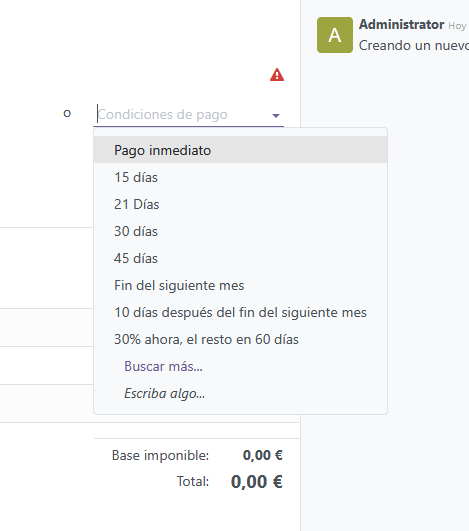
\includegraphics[width=0.8\textwidth]{pr2odoo05-facturac03.png}
    \caption{Condiciones de pago}
\end{figure}
\FloatBarrier

\begin{figure}[h!]
    \centering
    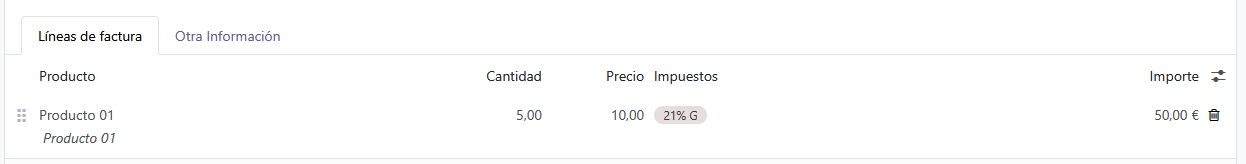
\includegraphics[width=1.2\textwidth]{pr2odoo06-facturac04.png}
    \caption{Productos}
\end{figure}
\FloatBarrier

\begin{figure}[h!]
    \centering
    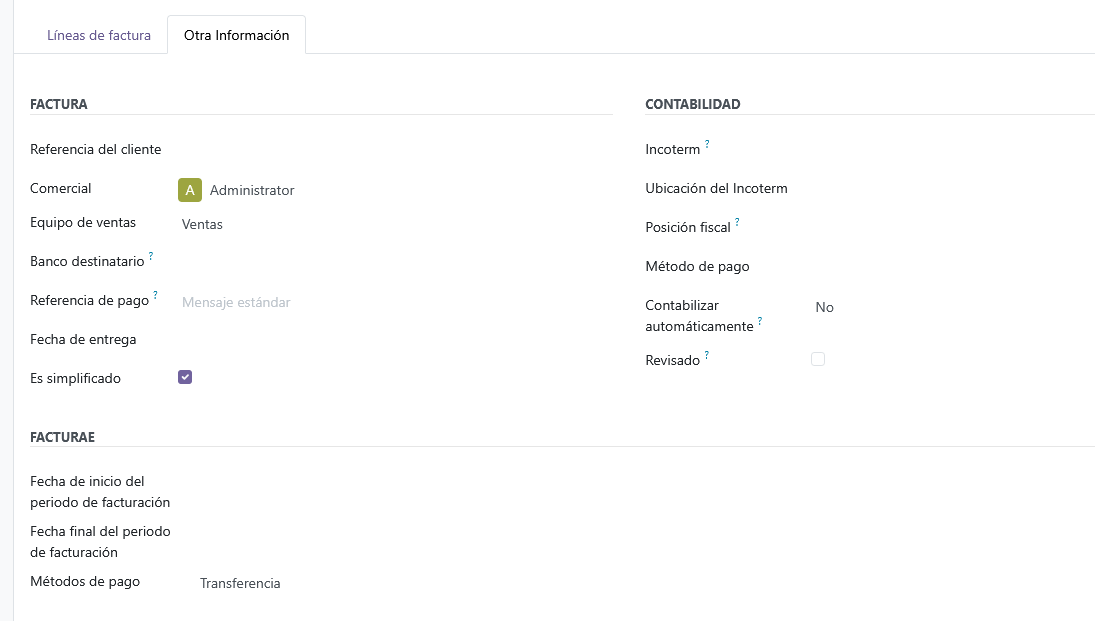
\includegraphics[width=1\textwidth]{pr2odoo07-facturac05.png}
    \caption{Otra información}
\end{figure}
\FloatBarrier

\begin{figure}[h!]
    \centering
    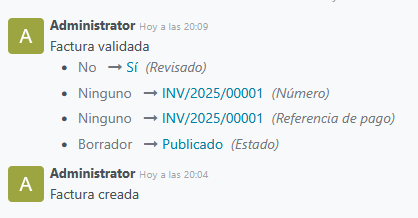
\includegraphics[width=0.8\textwidth]{pr2odoo08-facturac06.png}
    \caption{Resultado tras confirmar factura}
\end{figure}
\FloatBarrier

\begin{figure}[h!]
    \centering
    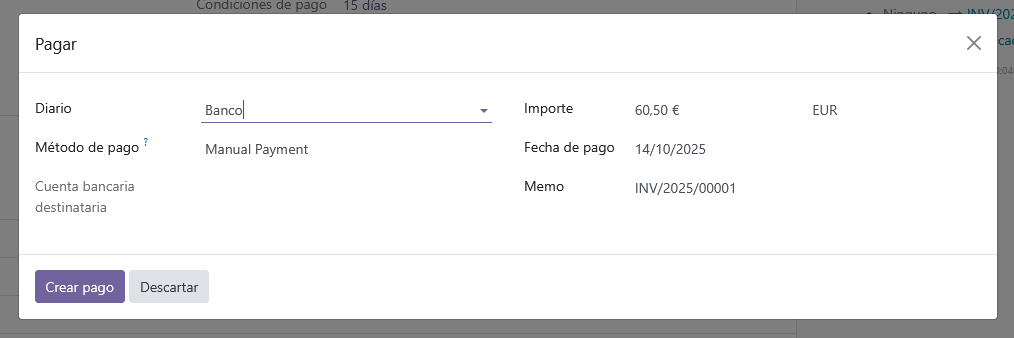
\includegraphics[width=1\textwidth]{pr2odoo09-facturac07.png}
    \caption{Pantalla de pago de factura}
\end{figure}
\FloatBarrier

\begin{figure}[h!]
    \centering
    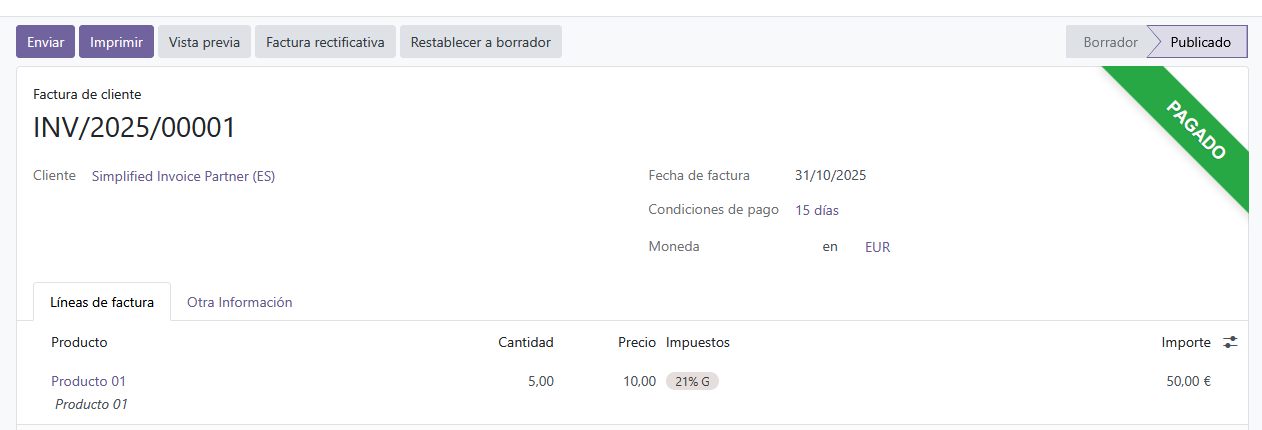
\includegraphics[width=1\textwidth]{pr2odoo10-facturac08.png}
    \caption{Factura pagada}
\end{figure}
\FloatBarrier

La pestaña Clientes permite organizar pagos, facturas, clientes y productos.

En Proveedores se manejan las facturas, reembolsos, pagos, productos y listas de los mismos, e Informes se ocupa del análisis de facturas.\\

Configuración permite editar:
\begin{enumerate}
    \item Condiciones de pago.
    \item Información bancaria.
    \item Contabilidad.
    \item Pagos en línea
    \item Categorías de productos.
\end{enumerate}

\clearpage

\subsection{Empleados}
\hyperlink{anchor-indice}{\textbf{Volver}}\\

El módulo de Empleados constituye el centro neurálgico de la gestión de recursos humanos con Odoo. Este nos permite llevar un control exhaustivo del ciclo de vida laboral de cada empleado, desde su incorporación hasta su potencial salida de la empresa.

Incluye herramientas para el control de asistencia y ausencias, la gestión de contratos y beneficios laborales, así como el seguimiento de evaluaciones de rendimiento y desarrollo profesional.

Su integración con otros módulos permite optimizar la planificación de recursos humanos y mejorar la eficiencia operativa de la organización.

\begin{figure}[h!]
    \centering
    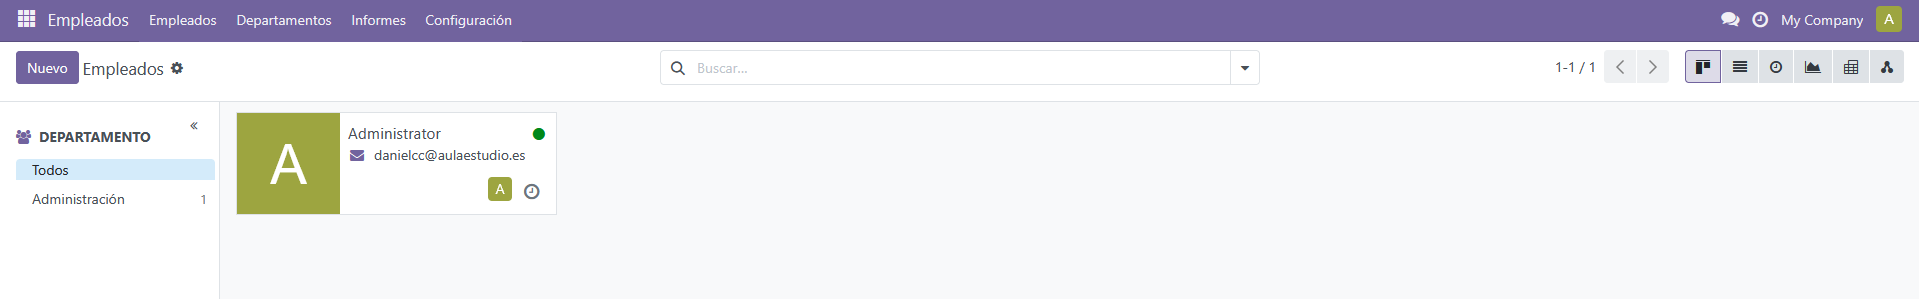
\includegraphics[width=1\textwidth]{pr2odoo11-empleadosMain.png}
    \caption{Pantalla principal de Empleados}
\end{figure}
\FloatBarrier

\begin{figure}[h!]
    \centering
    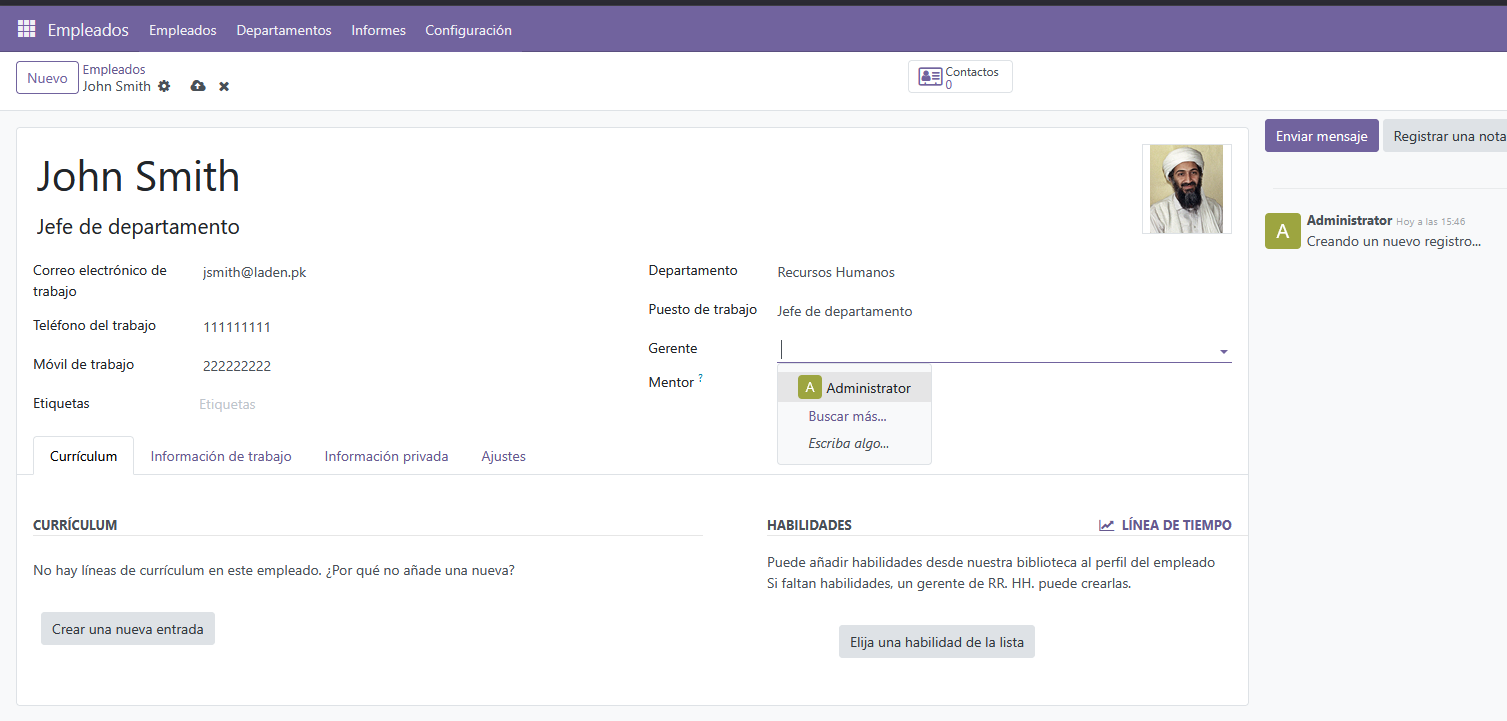
\includegraphics[width=1\textwidth]{pr2odoo12-DatosBasicosDeNuevoEmpleado.png}
    \caption{Datos básicos de nuevo empleado}
\end{figure}
\FloatBarrier

\begin{figure}[h!]
    \centering
    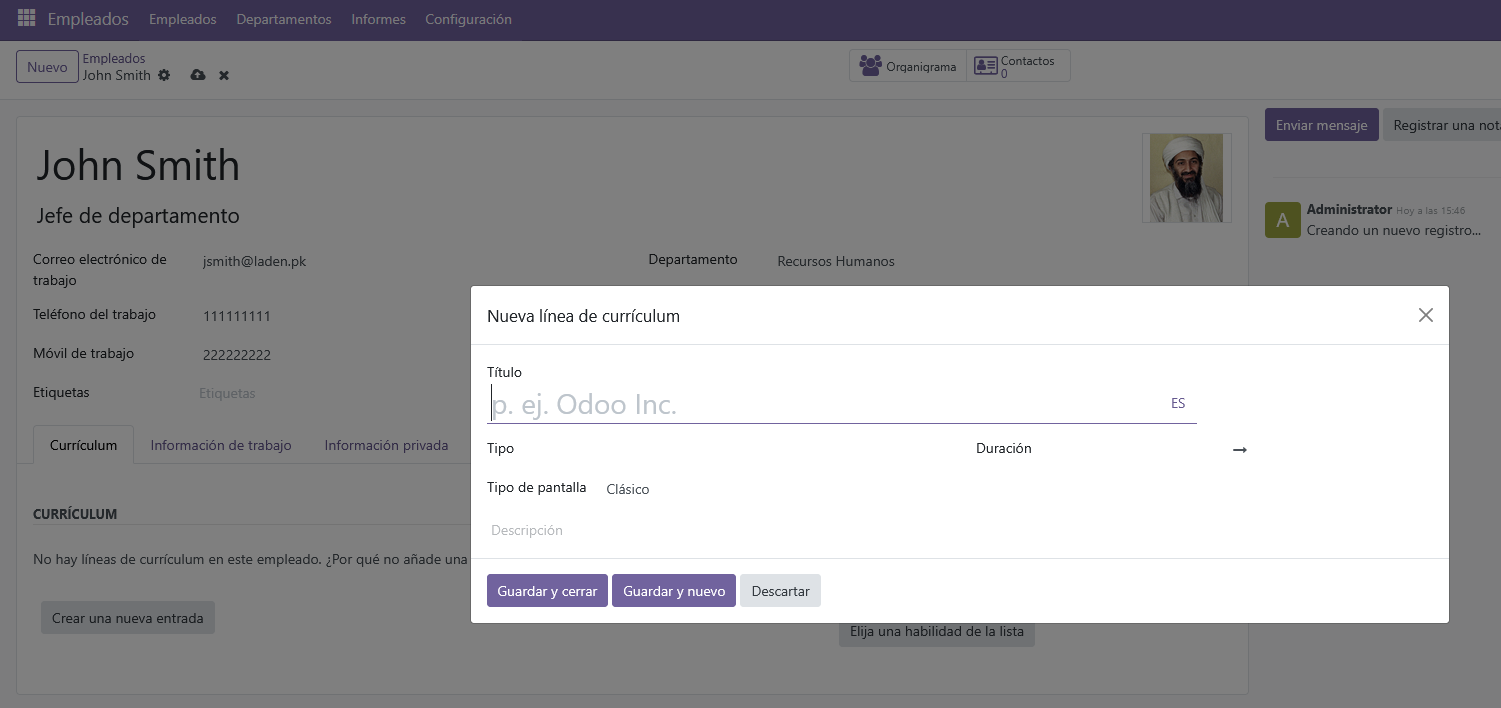
\includegraphics[width=1\textwidth]{pr2odoo13-curriculum.png}
    \caption{Curriculum}
\end{figure}
\FloatBarrier

\begin{figure}[h!]
    \centering
    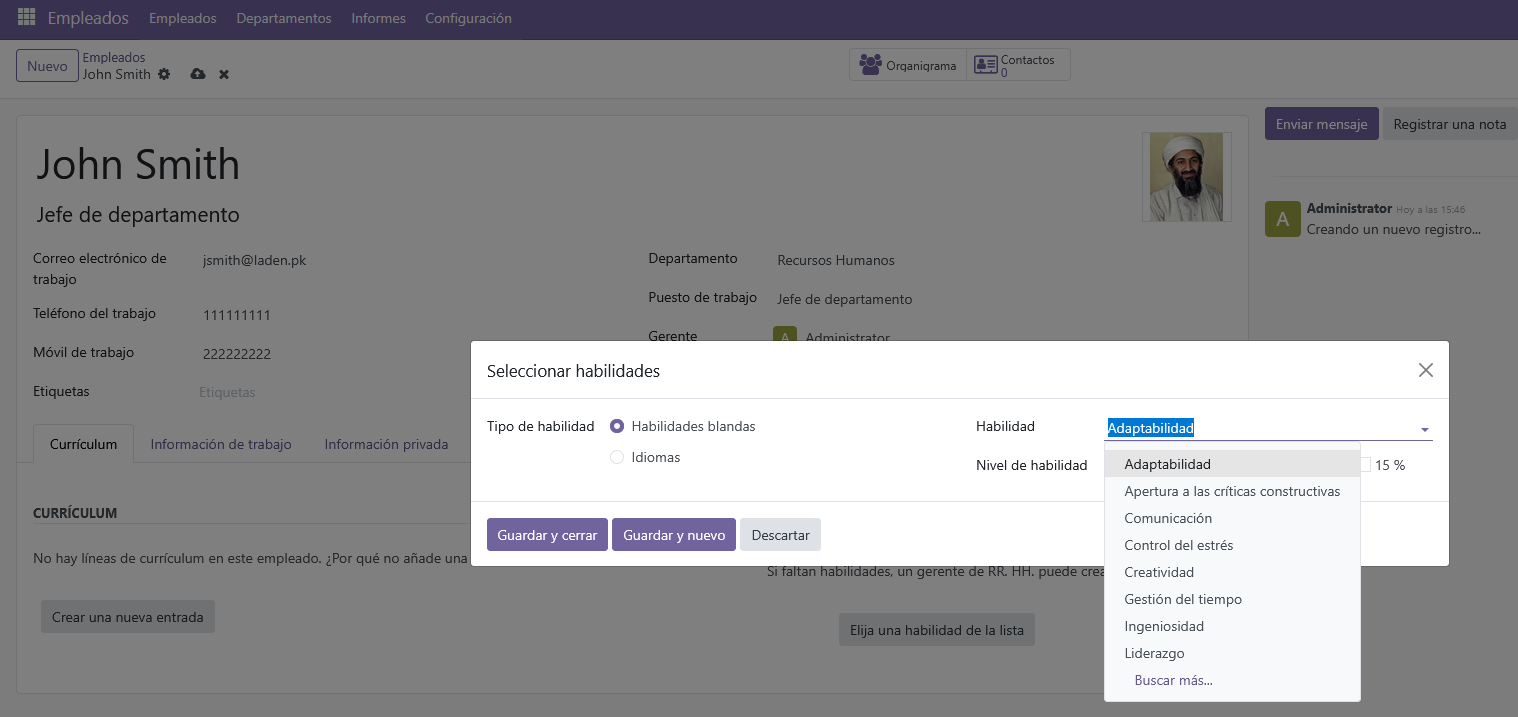
\includegraphics[width=1\textwidth]{pr2odoo14-habilidades.png}
    \caption{Habilidades}
\end{figure}
\FloatBarrier

\begin{figure}[h!]
    \centering
    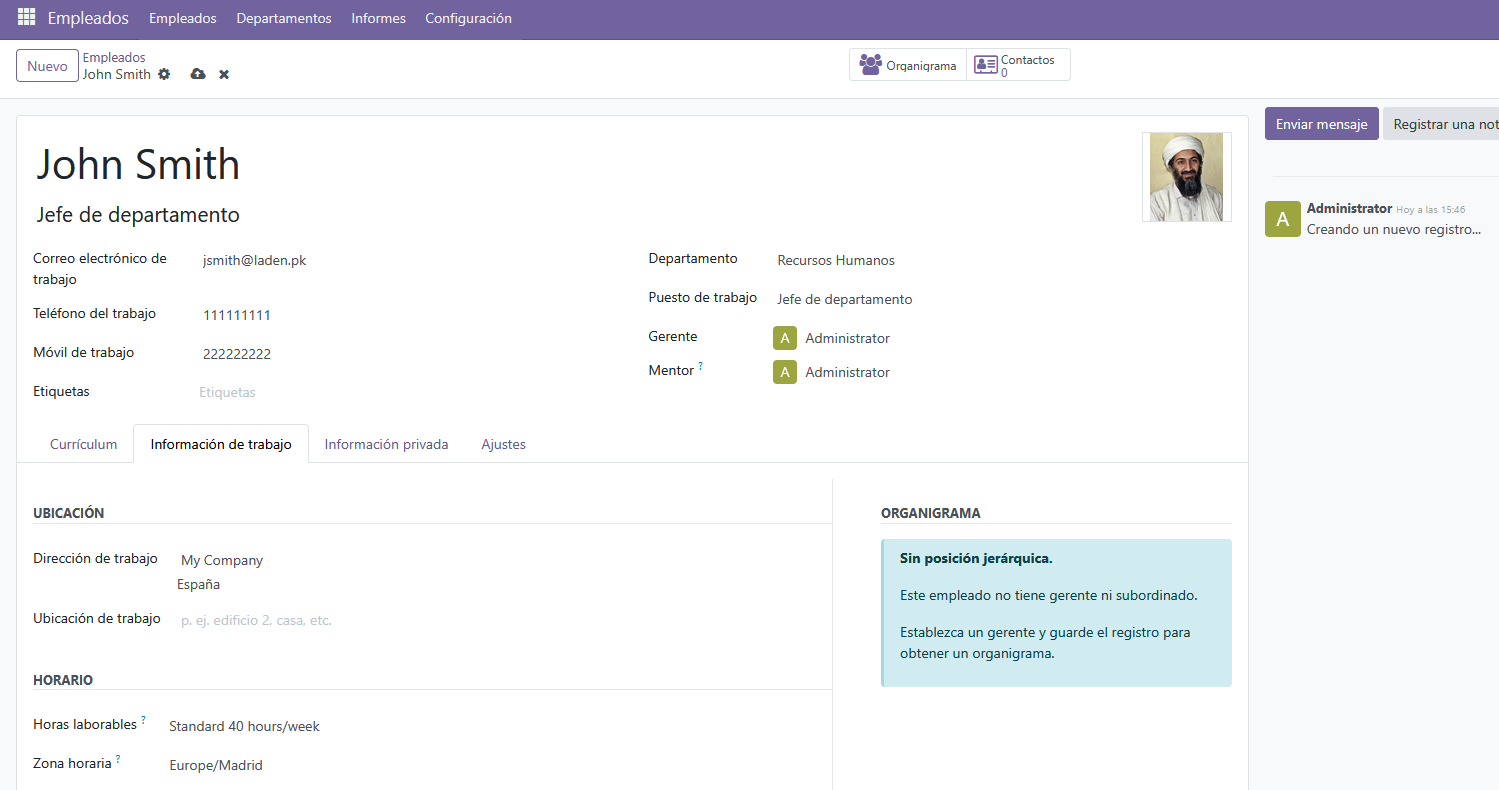
\includegraphics[width=1\textwidth]{pr2odoo15-informacionDeTrabajo.png}
    \caption{Información de trabajo}
\end{figure}
\FloatBarrier

\begin{figure}[h!]
    \centering
    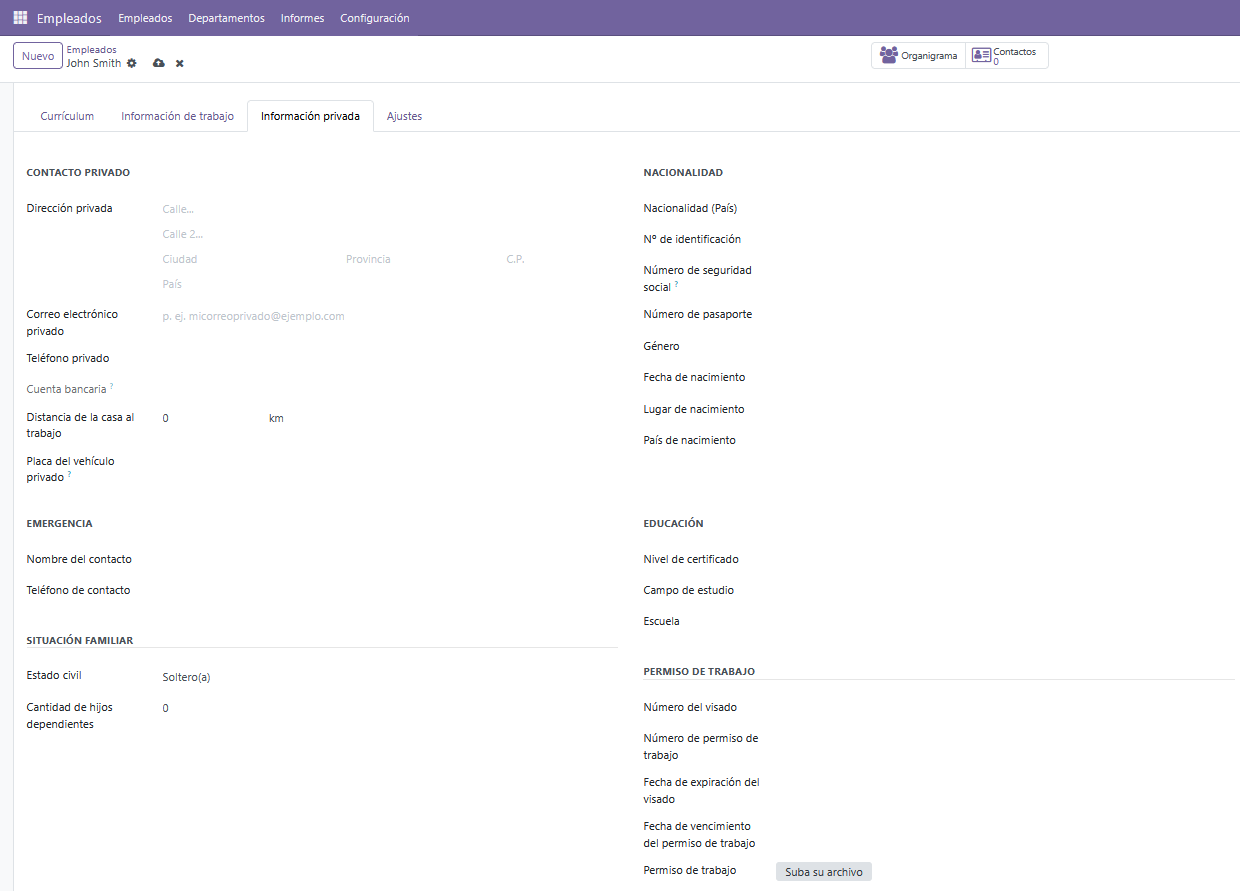
\includegraphics[width=1\textwidth]{pr2odoo16-informacionPrivada.png}
    \caption{Información privada}
\end{figure}
\FloatBarrier

\begin{figure}[h!]
    \centering
    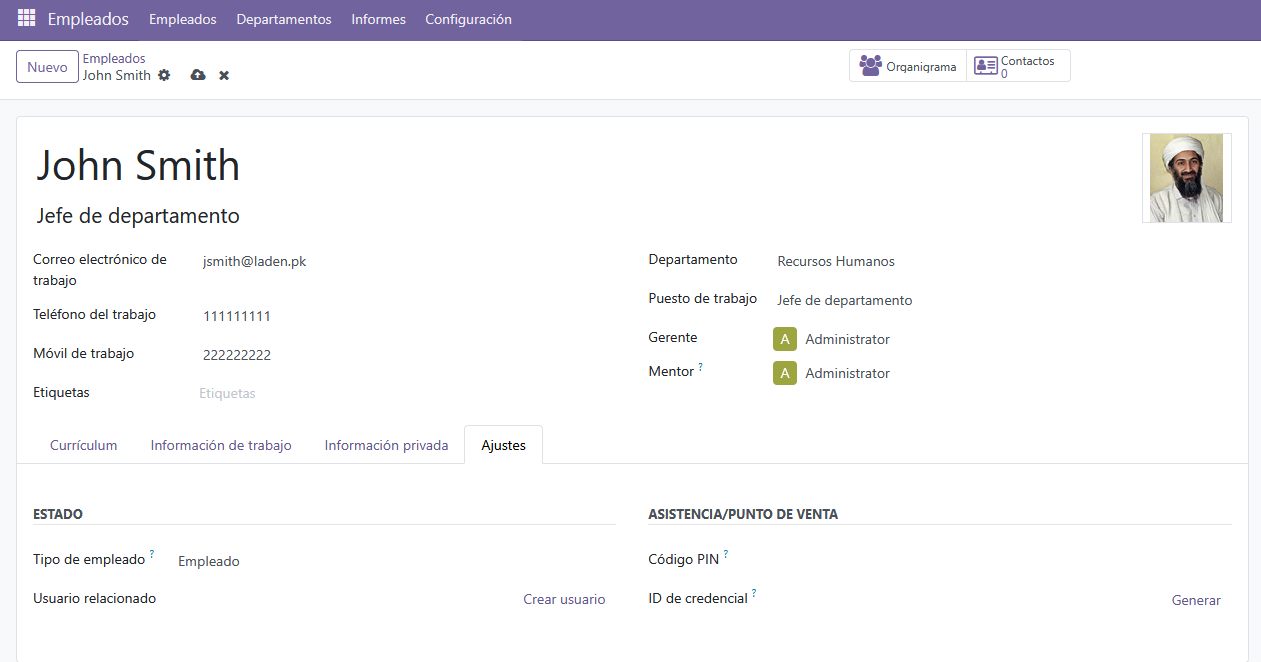
\includegraphics[width=1\textwidth]{pr2odoo17-ajustes.png}
    \caption{Ajustes}
\end{figure}
\FloatBarrier

\begin{figure}[h!]
    \centering
    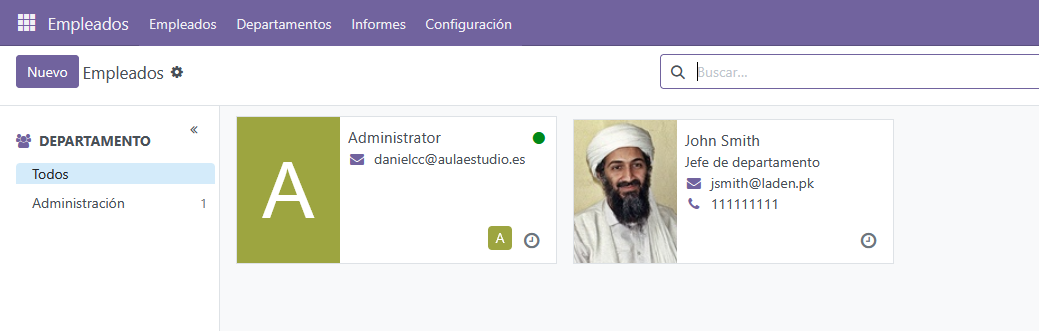
\includegraphics[width=1\textwidth]{pr2odoo18-empleadoCreado.png}
    \caption{Empleado creado}
\end{figure}
\FloatBarrier

\begin{figure}[h!]
    \centering
    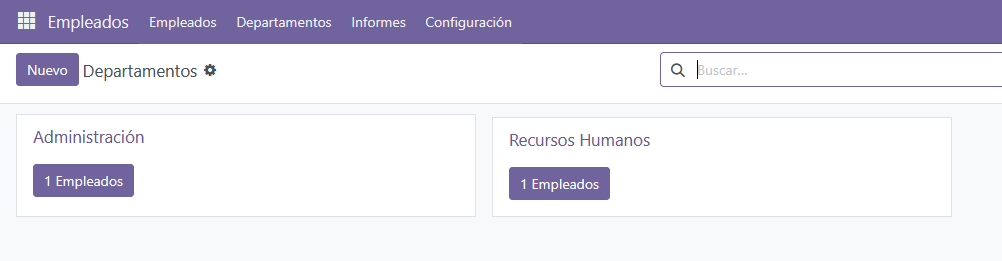
\includegraphics[width=1\textwidth]{pr2odoo19-departamentos.png}
    \caption{Departamentos actuales}
\end{figure}
\FloatBarrier

\begin{figure}[h!]
    \centering
    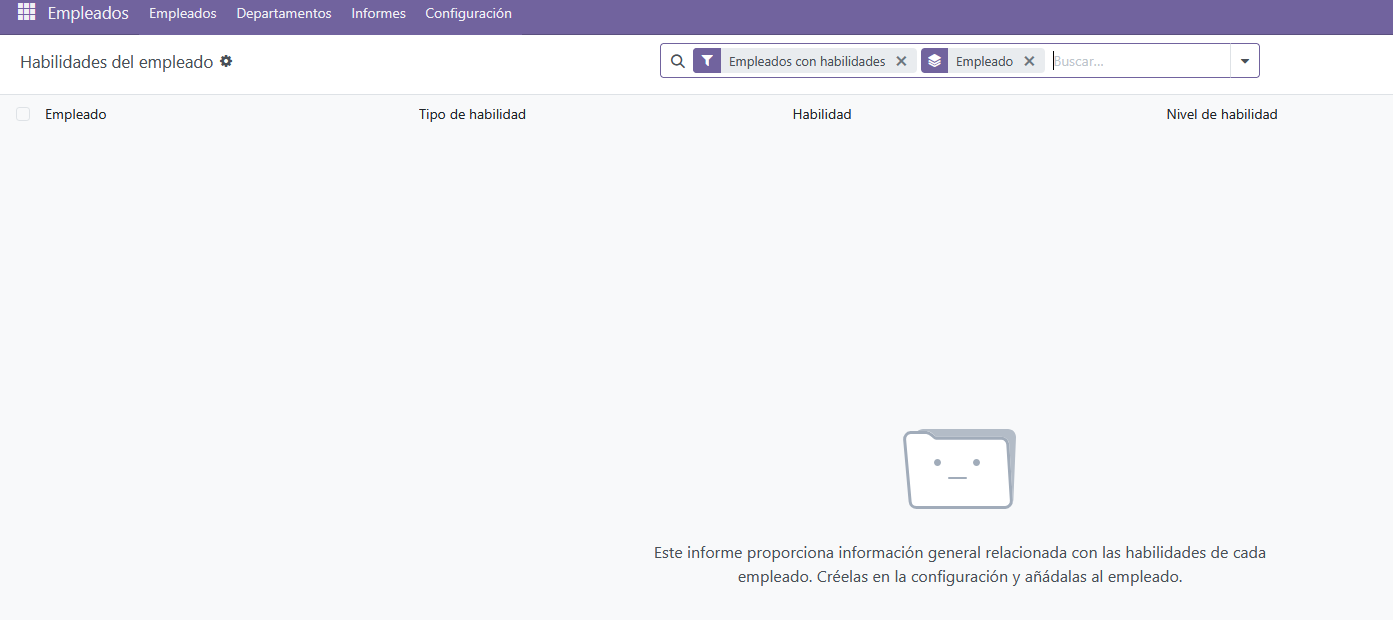
\includegraphics[width=1\textwidth]{pr2odoo20-habilidadesDeEmpleado.png}
    \caption{Habilidades de empleado}
\end{figure}
\FloatBarrier

\begin{figure}[h!]
    \centering
    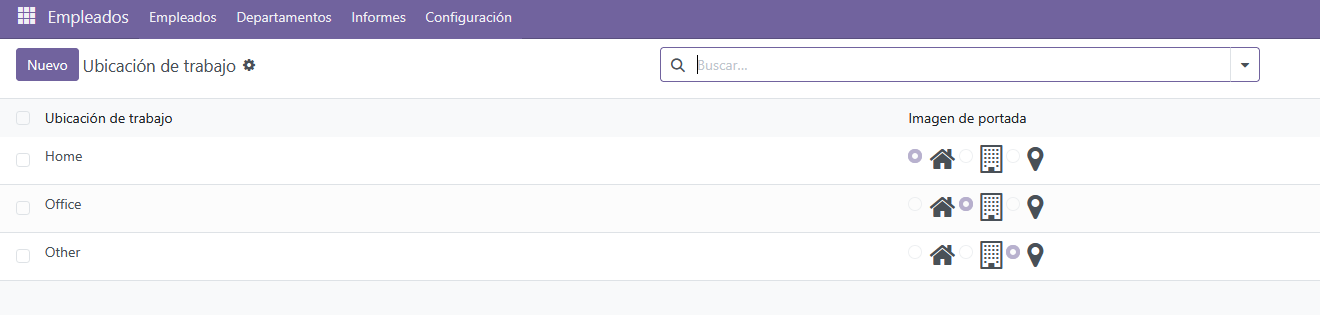
\includegraphics[width=1\textwidth]{pr2odoo21-ubicacionDeTrabajo.png}
    \caption{Ubicación de trabajo}
\end{figure}
\FloatBarrier

\begin{figure}[h!]
    \centering
    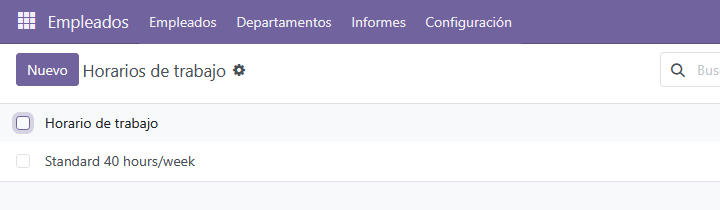
\includegraphics[width=1\textwidth]{pr2odoo22-horarios.png}
    \caption{Horarios de trabajo}
\end{figure}
\FloatBarrier

\begin{figure}[h!]
    \centering
    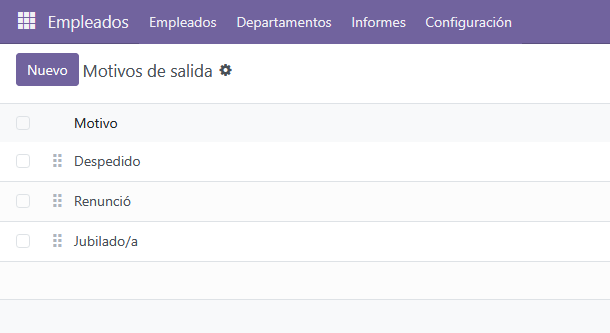
\includegraphics[width=1\textwidth]{pr2odoo23-motivosSalida.png}
    \caption{Motivos de salida}
\end{figure}
\FloatBarrier

\begin{figure}[h!]
    \centering
    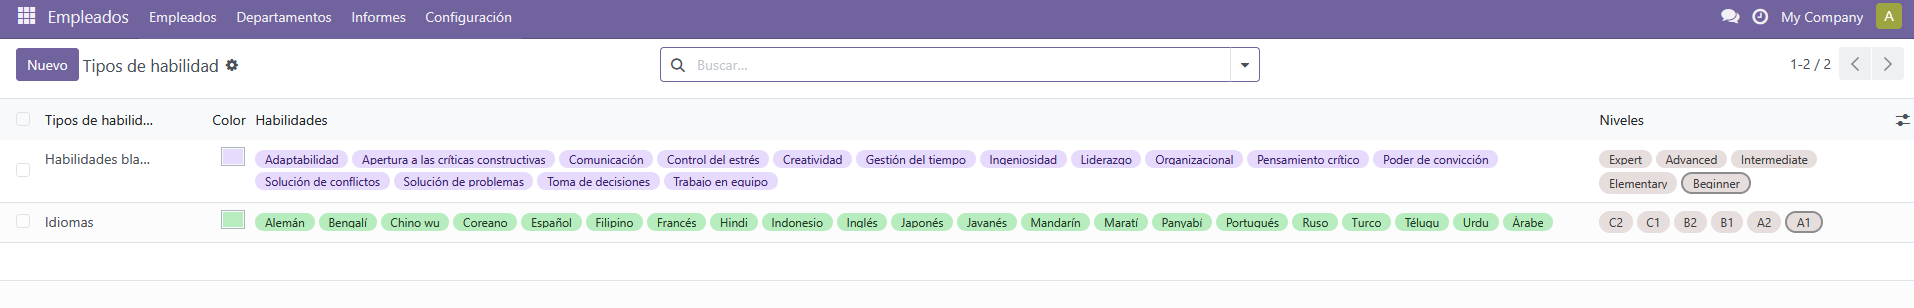
\includegraphics[width=1\textwidth]{pr2odoo24-tiposHabilidad.png}
    \caption{Tipos de habilidad}
\end{figure}
\FloatBarrier

\begin{figure}[h!]
    \centering
    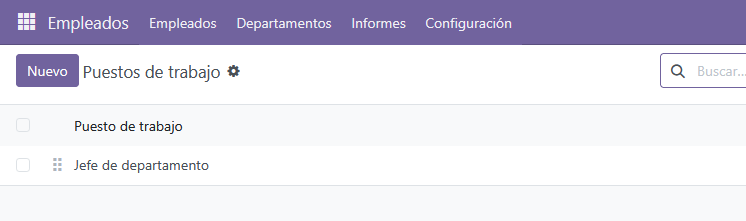
\includegraphics[width=1\textwidth]{pr2odoo25-puestosTrabajo.png}
    \caption{Puestos de trabajo}
\end{figure}
\FloatBarrier

\begin{figure}[h!]
    \centering
    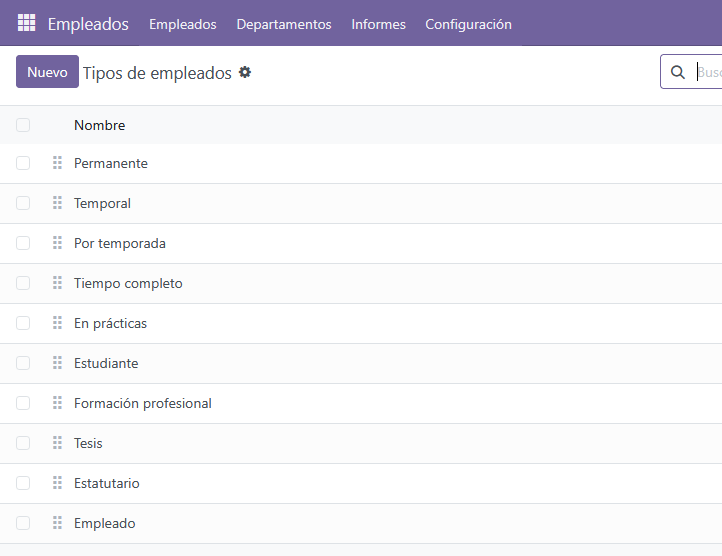
\includegraphics[width=1\textwidth]{pr2odoo26-tiposEmpleado.png}
    \caption{Tipos de empleado}
\end{figure}
\FloatBarrier

Las pestañas de Empleados, Departamentos e Informes llevan a su sección correspondiente.

Configuración permite editar el plan de actividad, la información de empleados y de reclutamiento.

\clearpage

\subsection{Compras}
\hyperlink{anchor-indice}{\textbf{Volver}}\\

El módulo de Compras es esencial para la gestión de la cadena de suministros. Permite centralizar y optimizar todo el proceso de compras, desde la solicitud inicial hasta la recepción de la mercancía.

Una de sus características más importantes es la capacidad de establecer reglas de reposición automática del inventario, lo que ayuda a mantener niveles óptimos de stock y evitar falta o exceso de inventario.

Además, facilita la negociación con proveedores y el análisis comparativo de precios, contribuyendo así a la reducción de costos y mejora de la rentabilidad.

\begin{figure}[h!]
    \centering
    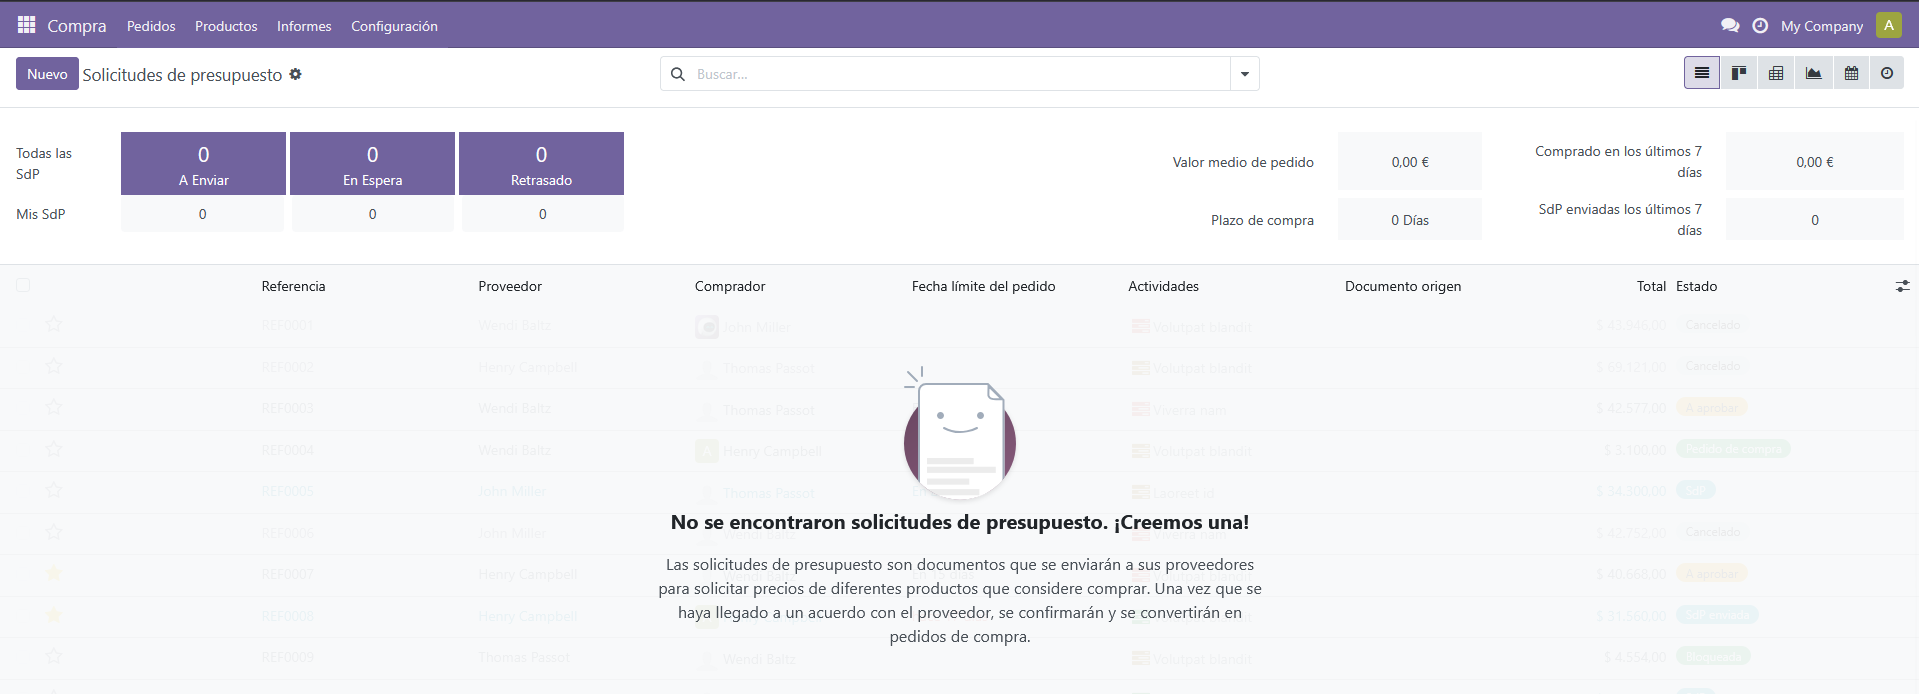
\includegraphics[width=1\textwidth]{pr2odoo27-pantallaPrincipalCompras.png}
    \caption{Pantalla principal de compras}
\end{figure}
\FloatBarrier

\begin{figure}[h!]
    \centering
    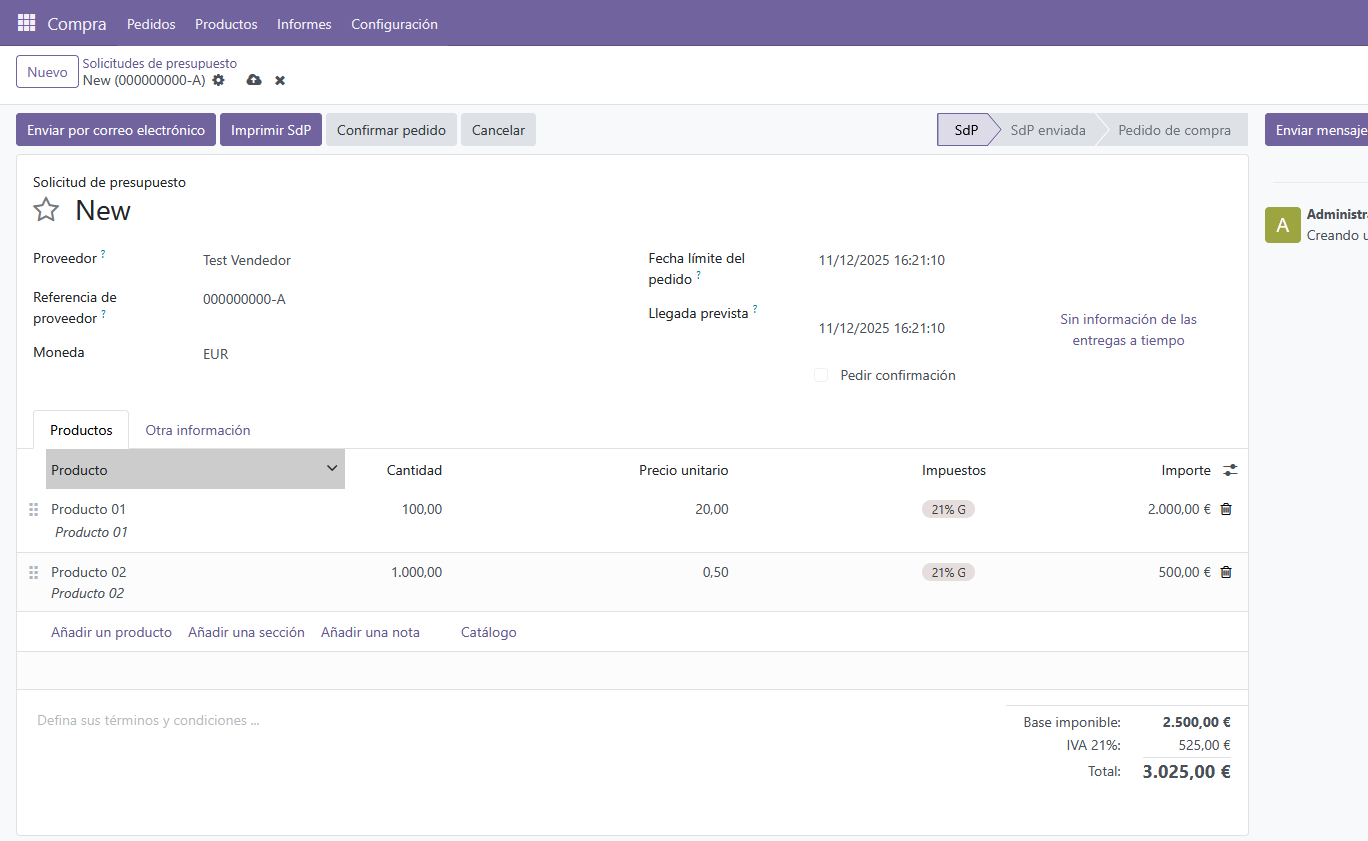
\includegraphics[width=1\textwidth]{pr2odoo28-nuevoPresupuesto.png}
    \caption{Nuevo presupuesto: información básica y productos}
\end{figure}
\FloatBarrier

\begin{figure}[h!]
    \centering
    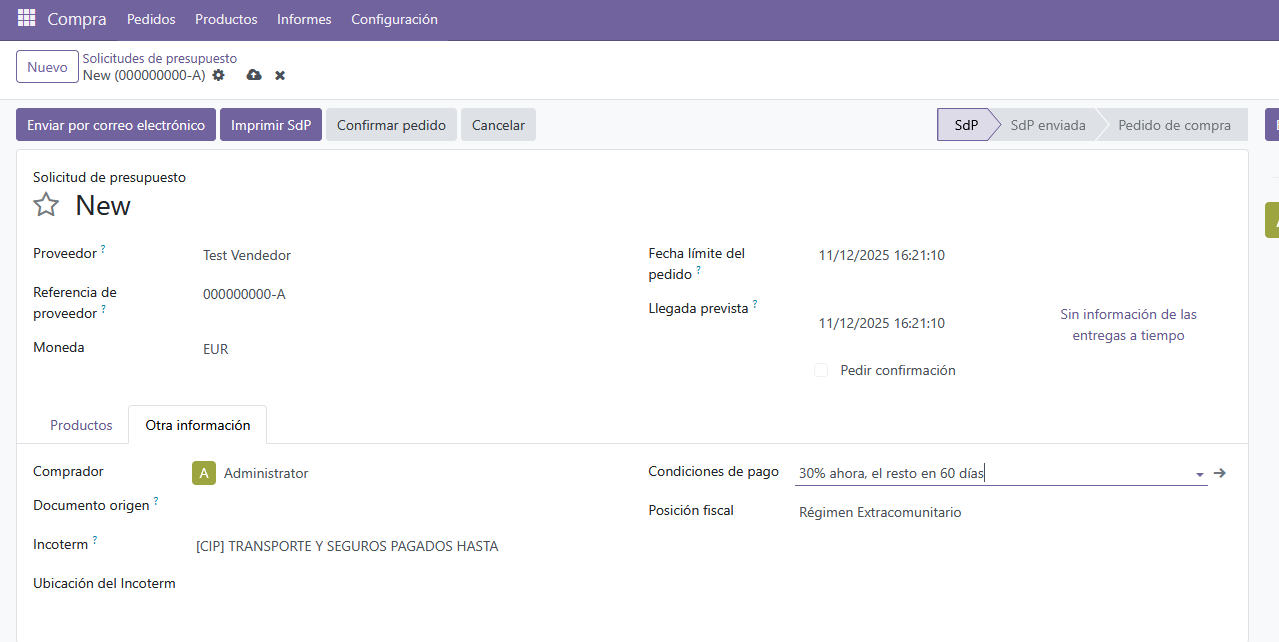
\includegraphics[width=1\textwidth]{pr2odoo29-otraInfo.png}
    \caption{Otra información}
\end{figure}
\FloatBarrier

\begin{figure}[h!]
    \centering
    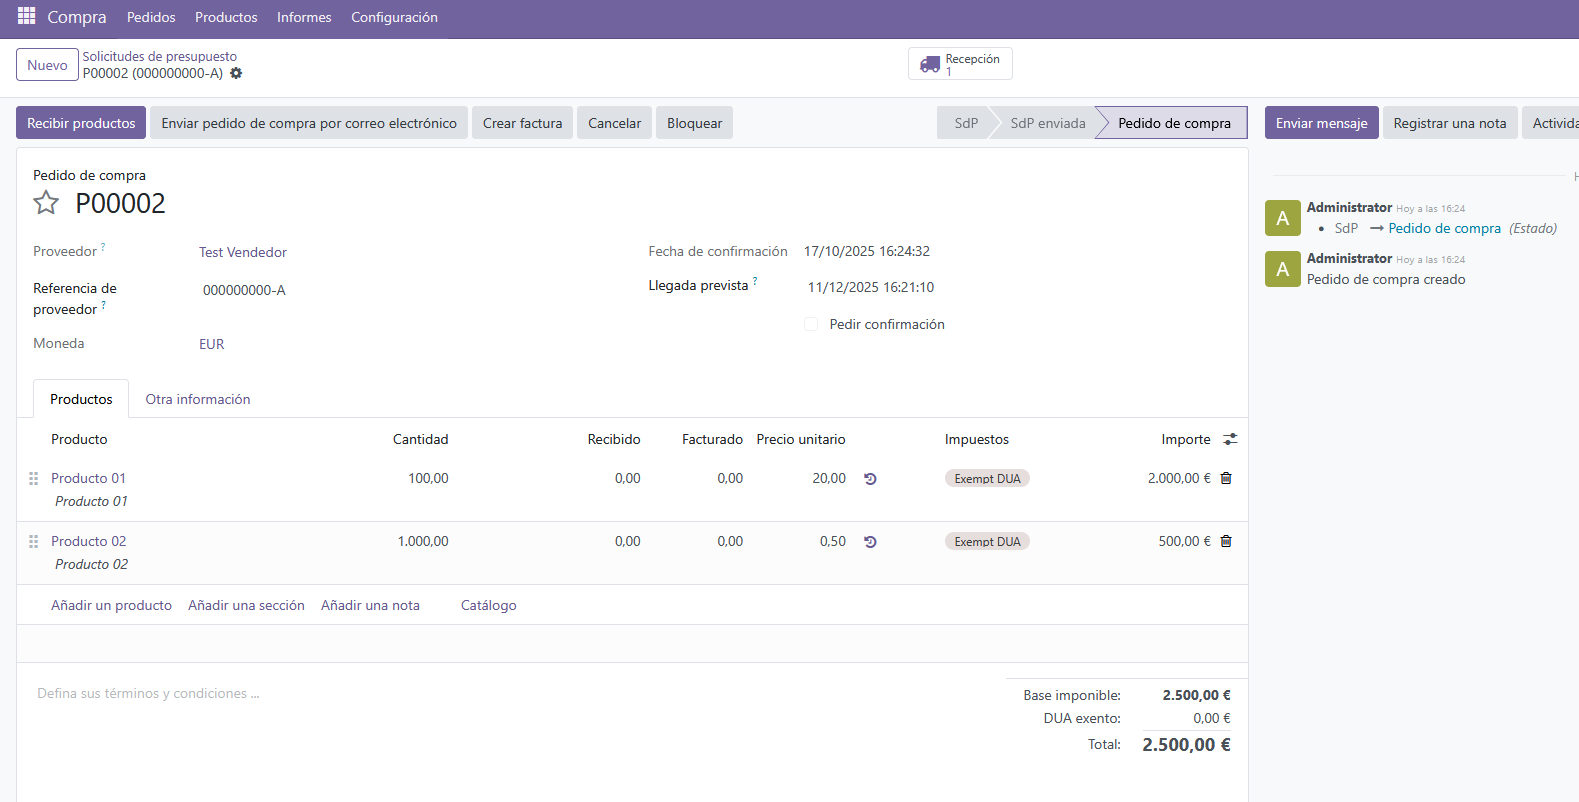
\includegraphics[width=1\textwidth]{pr2odoo30-pedidoCreado.png}
    \caption{Pedido creado}
\end{figure}
\FloatBarrier

\begin{figure}[h!]
    \centering
    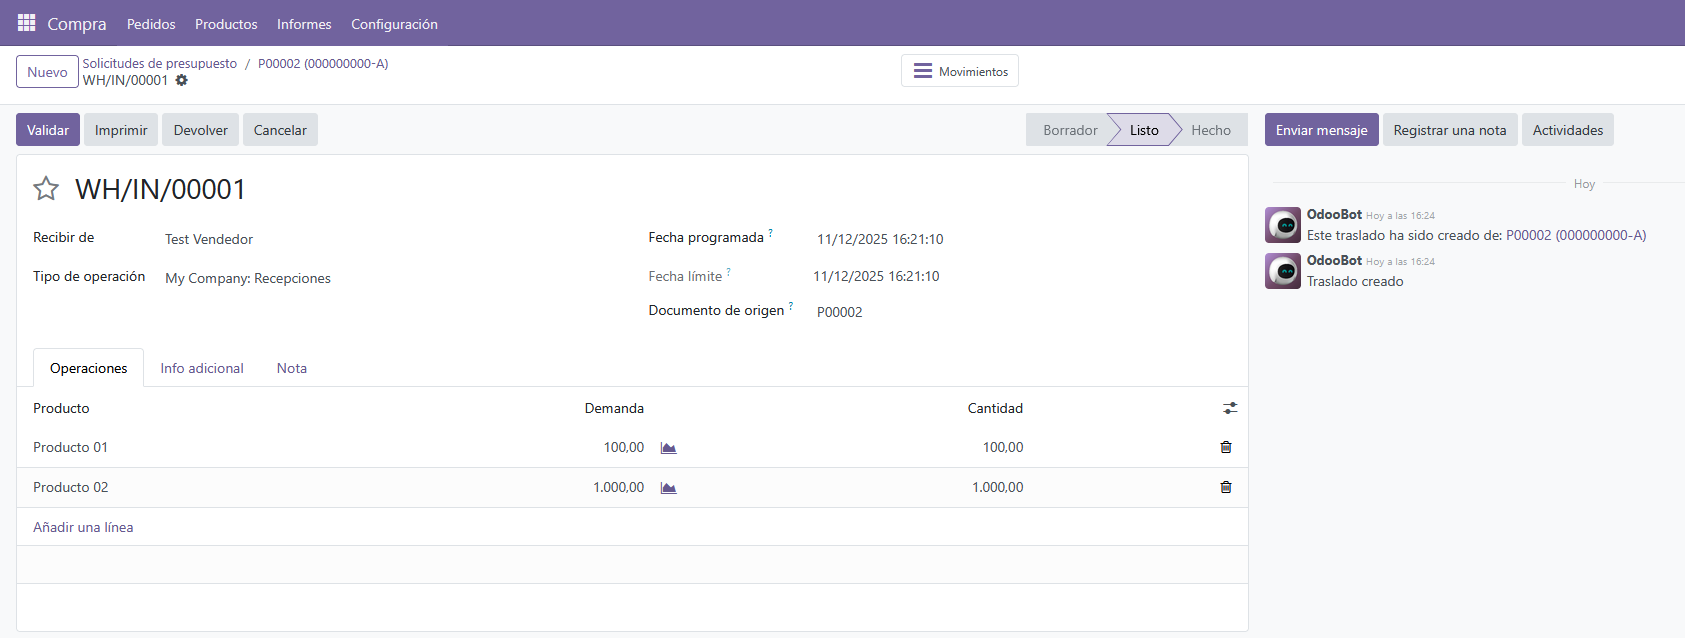
\includegraphics[width=1\textwidth]{pr2odoo31-productosRecibidos.png}
    \caption{Productos recibidos}
\end{figure}
\FloatBarrier

\begin{figure}[h!]
    \centering
    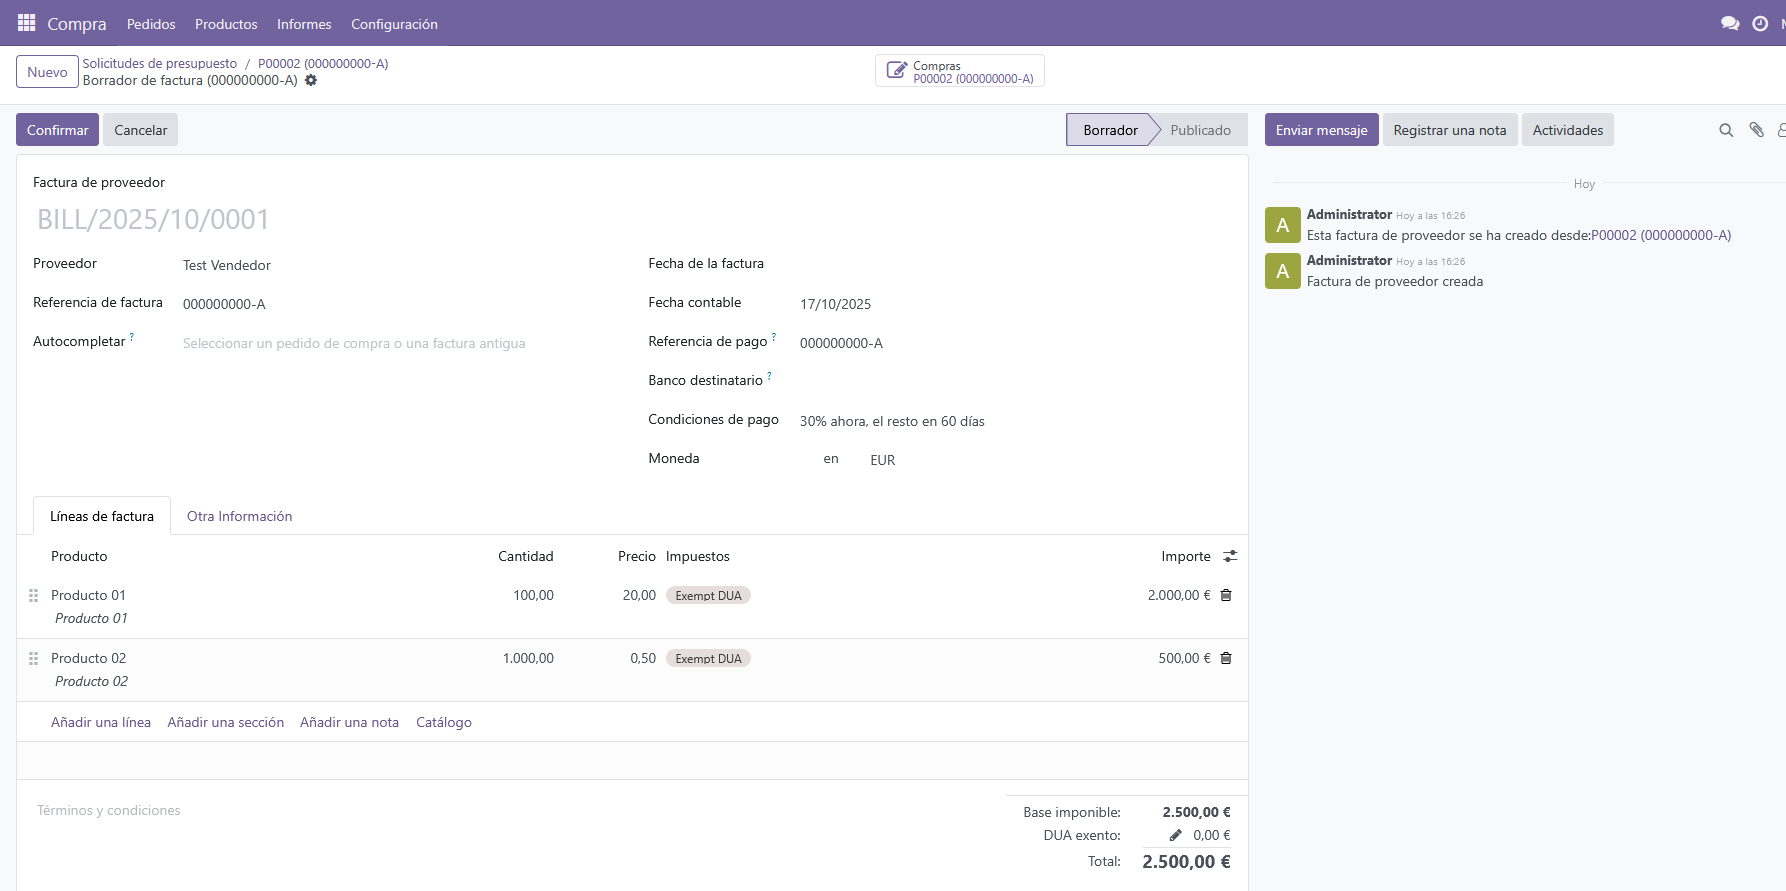
\includegraphics[width=1\textwidth]{pr2odoo32-facturaProveedorCreada.png}
    \caption{Factura de proveedor creada}
\end{figure}
\FloatBarrier

\begin{figure}[h!]
    \centering
    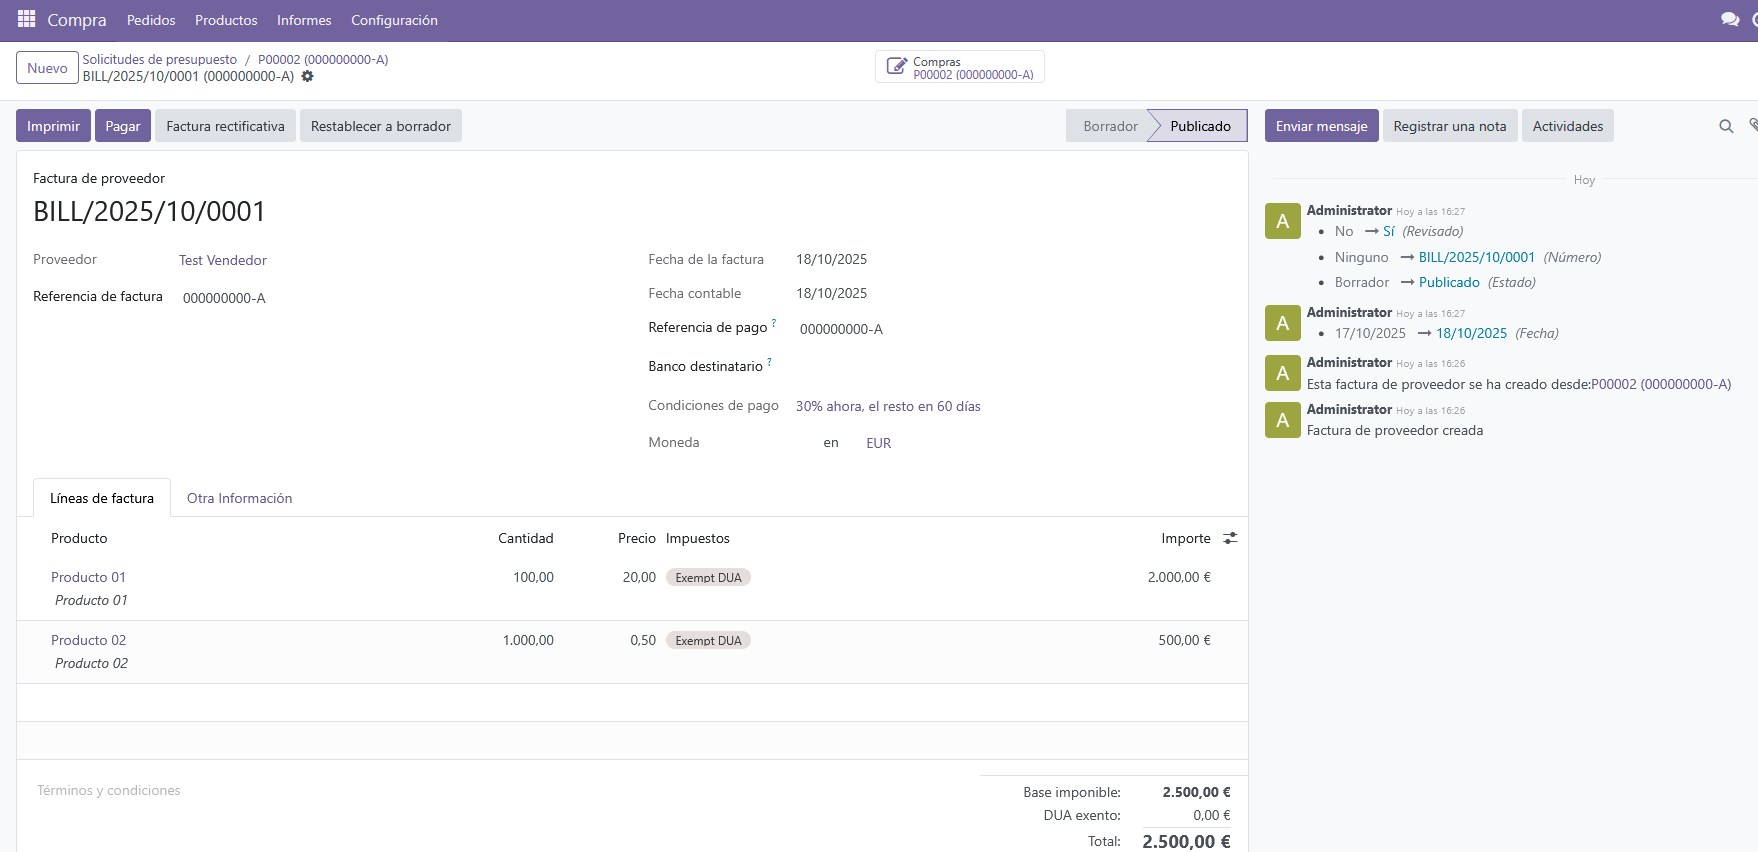
\includegraphics[width=1\textwidth]{pr2odoo33-preparadaParaPago.png}
    \caption{Factura preparada para pago}
\end{figure}
\FloatBarrier

\begin{figure}[h!]
    \centering
    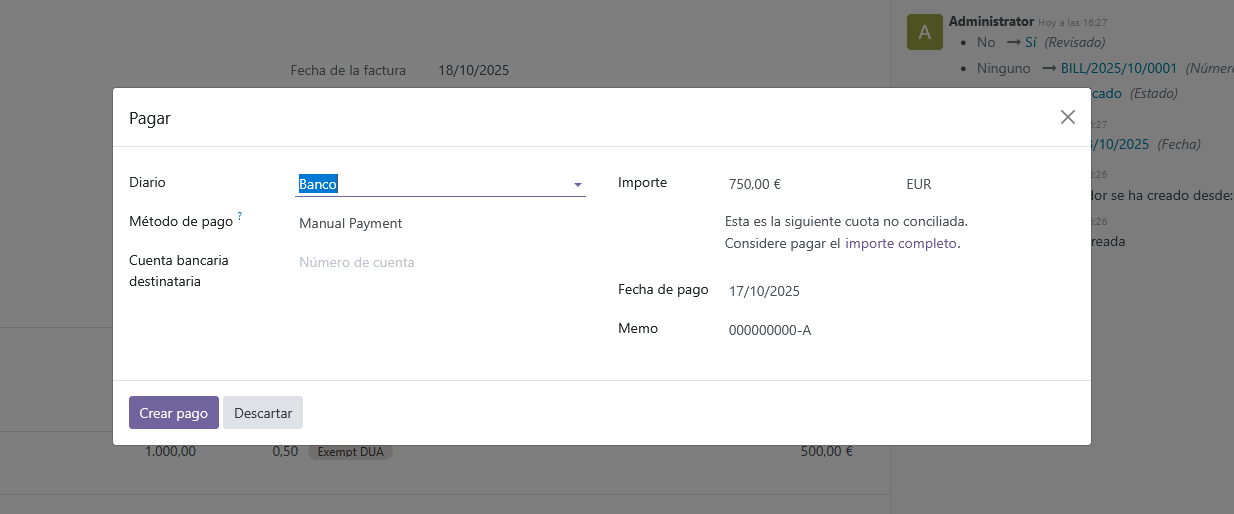
\includegraphics[width=1\textwidth]{pr2odoo34-pantallaPago.png}
    \caption{Pantalla de pago}
\end{figure}
\FloatBarrier

\begin{figure}[h!]
    \centering
    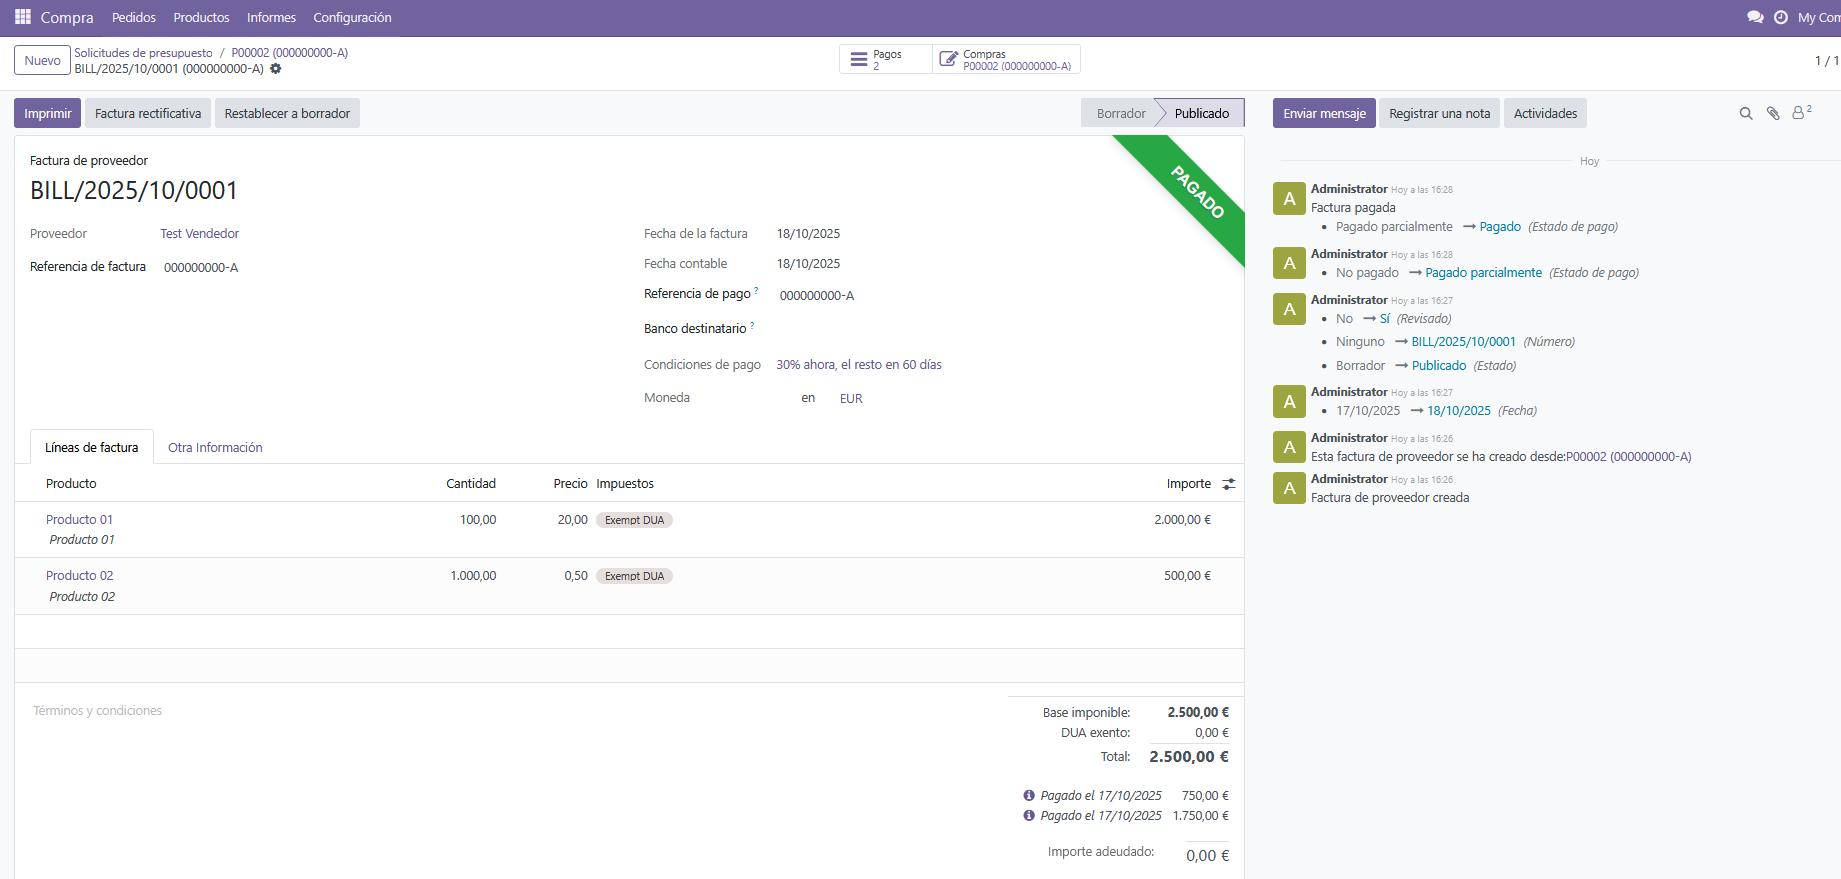
\includegraphics[width=1\textwidth]{pr2odoo35-facturaPagada.png}
    \caption{Factura pagada}
\end{figure}
\FloatBarrier

\begin{figure}[h!]
    \centering
    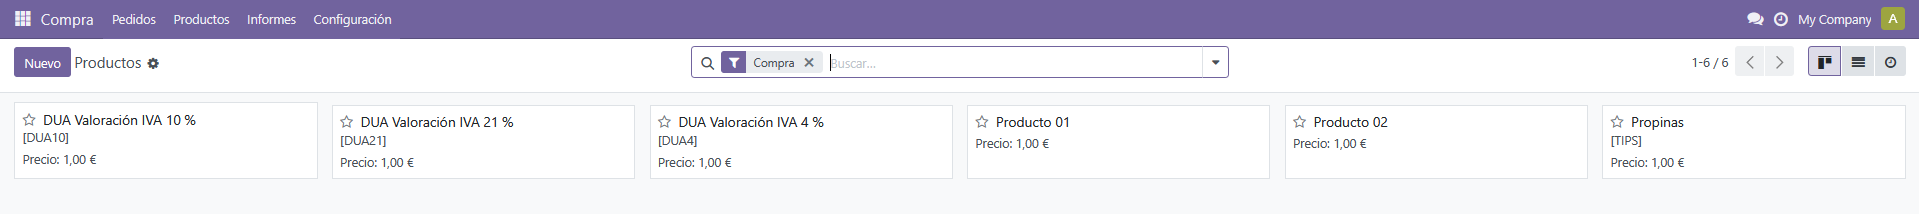
\includegraphics[width=1\textwidth]{pr2odoo36-pantallaProductos.png}
    \caption{Pantalla de productos}
\end{figure}
\FloatBarrier

\begin{figure}[h!]
    \centering
    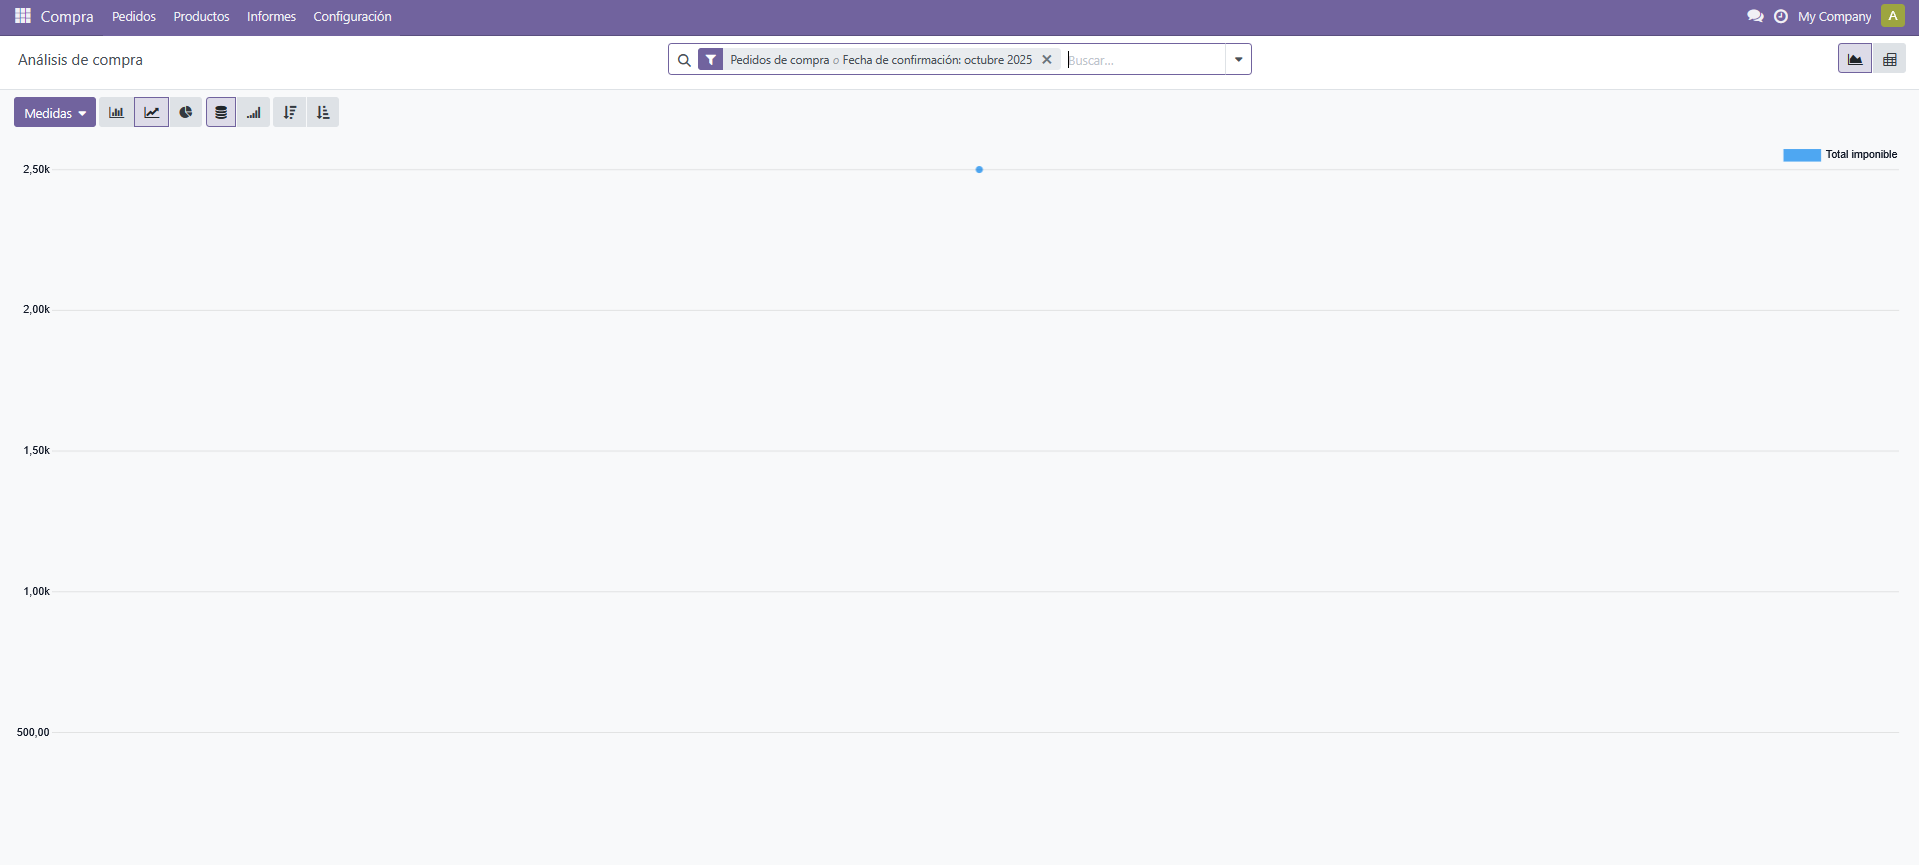
\includegraphics[width=1\textwidth]{pr2odoo37-analisisCompras.png}
    \caption{Pantalla de informes de análisis de compras}
\end{figure}
\FloatBarrier

\begin{figure}[h!]
    \centering
    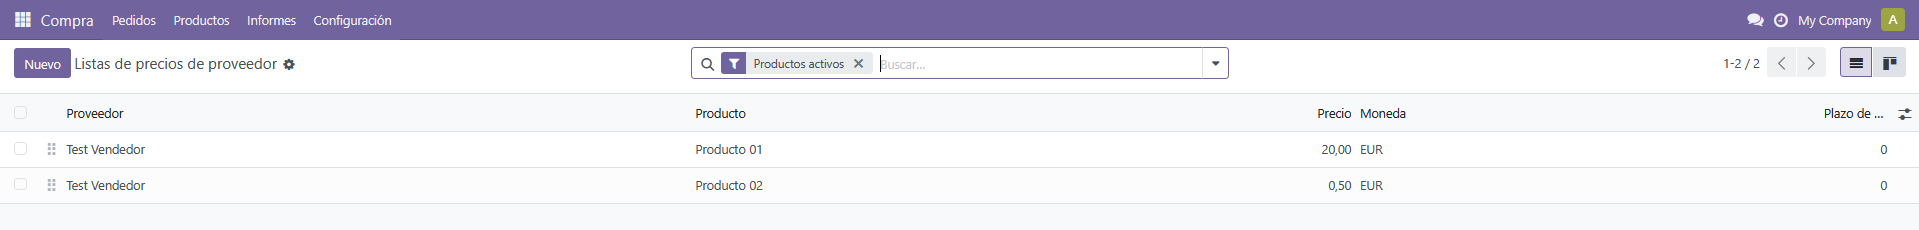
\includegraphics[width=1\textwidth]{pr2odoo38-preciosProveedor.png}
    \caption{Lista de precios de proveedores}
\end{figure}
\FloatBarrier

\begin{figure}[h!]
    \centering
    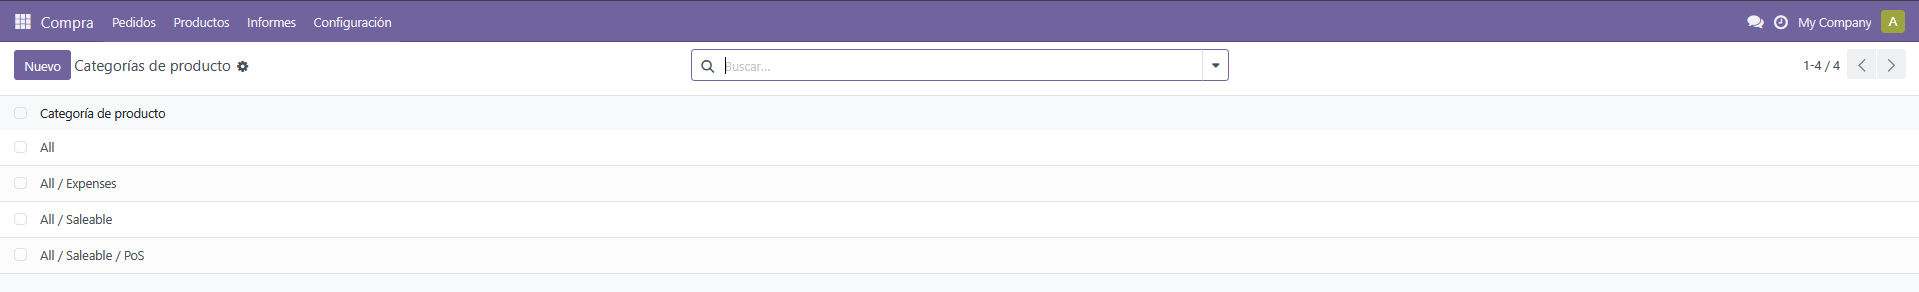
\includegraphics[width=1\textwidth]{pr2odoo39-categoriasPrioductos.png}
    \caption{Categorías de productos}
\end{figure}
\FloatBarrier

Las pestañas de Pedidos, Productos e Informes llevan a su sección correspondiente.

Configuración permite editar las listas de precios de proveedor y las categorías de productos.

\clearpage

\subsection{Ventas}
\hyperlink{anchor-indice}{\textbf{Volver}}\\

El módulo de Ventas es otro de los pilares de Odoo, proporcionando herramientas avanzadas para gestionar todo el proceso de ventas, desde la captación de leads hasta la entrega final del producto.

Ofrece capacidades robustas para crear y gestionar cotizaciones, convertir oportunidades en ventas, y realizar un seguimiento detallado de pedidos y entregas.

Su integración con el módulo CRM permite mantener una visión completa del cliente y personalizar la experiencia comercial según las necesidades específicas y comportamiento de compra.

\begin{figure}[h!]
    \centering
    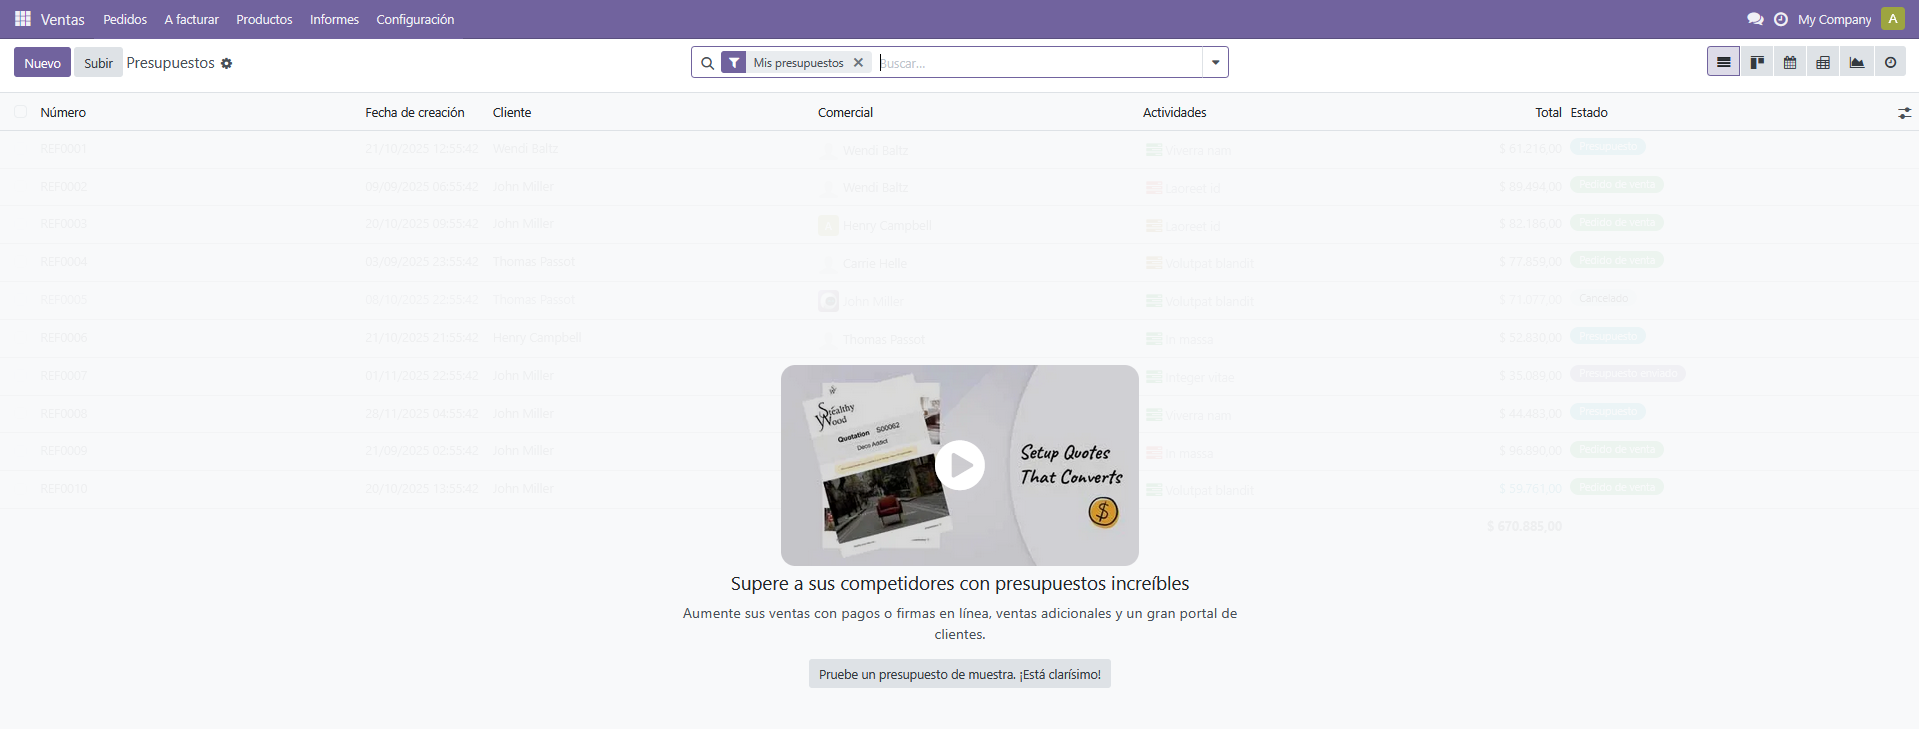
\includegraphics[width=1\textwidth]{pr2odoo40-pantallaPrincipalVentas.png}
    \caption{Pantalla principal de ventas}
\end{figure}
\FloatBarrier

\begin{figure}[h!]
    \centering
    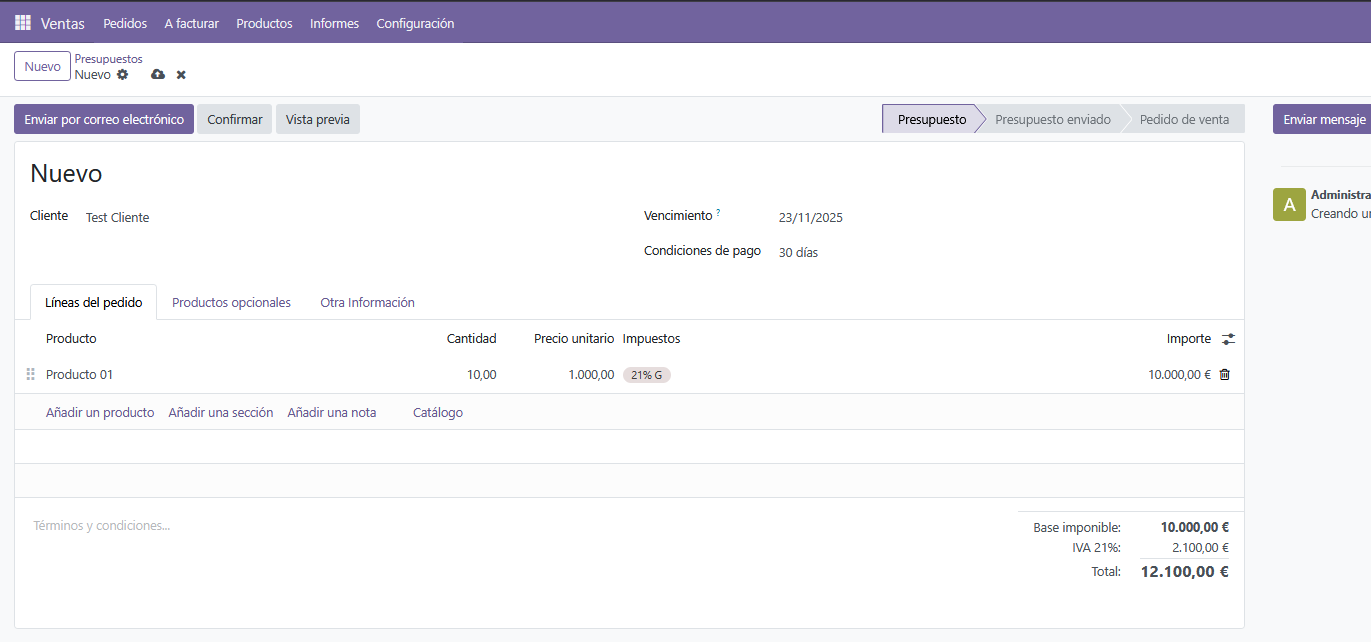
\includegraphics[width=1\textwidth]{pr2odoo41-nuevoPresupuesto.png}
    \caption{Nuevo presupuesto de venta}
\end{figure}
\FloatBarrier

\begin{figure}[h!]
    \centering
    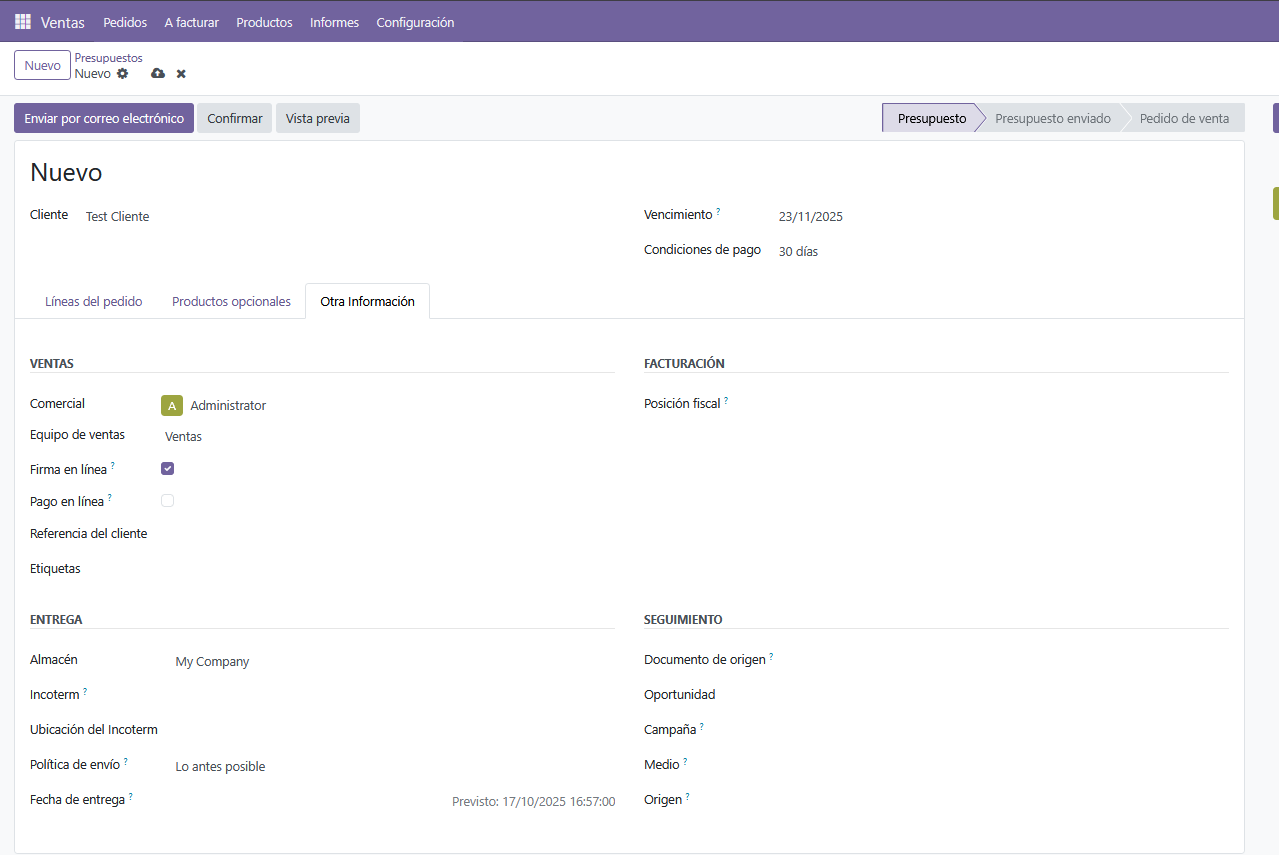
\includegraphics[width=1\textwidth]{pr2odoo42-otraInfo.png}
    \caption{Otra información}
\end{figure}
\FloatBarrier

\begin{figure}[h!]
    \centering
    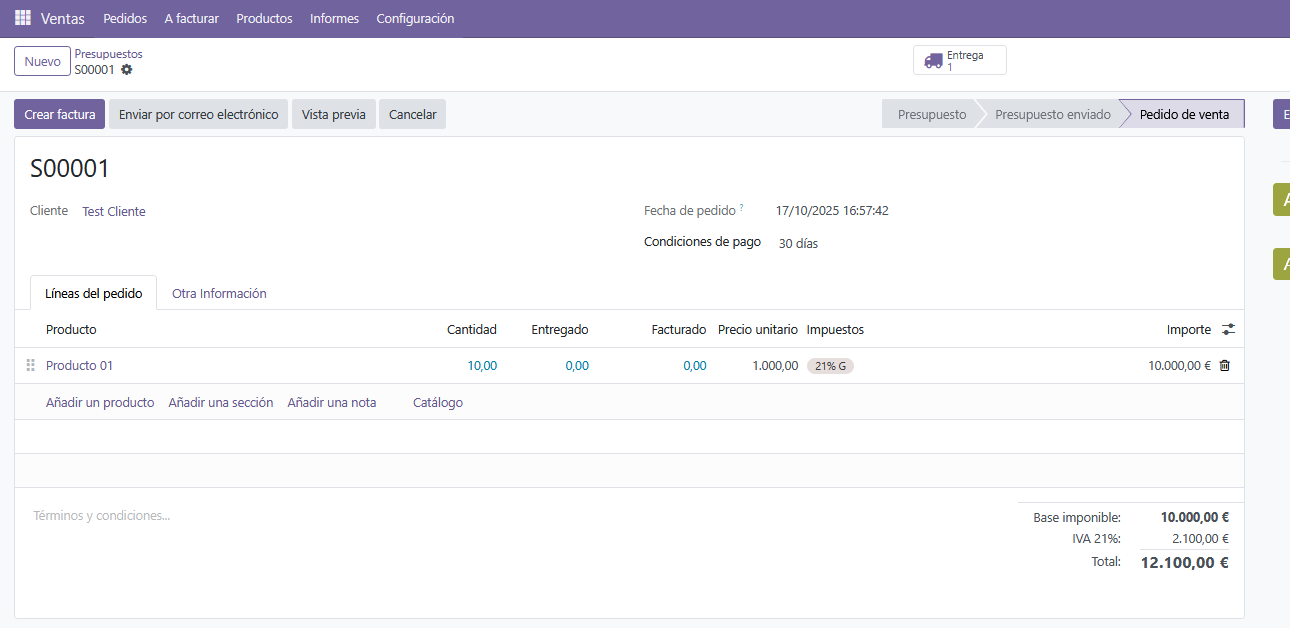
\includegraphics[width=1\textwidth]{pr2odoo43-presupuestoCreado.png}
    \caption{Presupuesto creado}
\end{figure}
\FloatBarrier

\begin{figure}[h!]
    \centering
    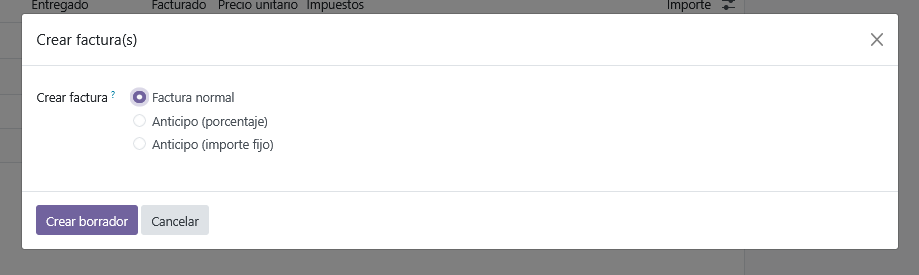
\includegraphics[width=1\textwidth]{pr2odoo44-crearBorradorFactura.png}
    \caption{Pantalla de creación de borrador de factura}
\end{figure}
\FloatBarrier

\begin{figure}[h!]
    \centering
    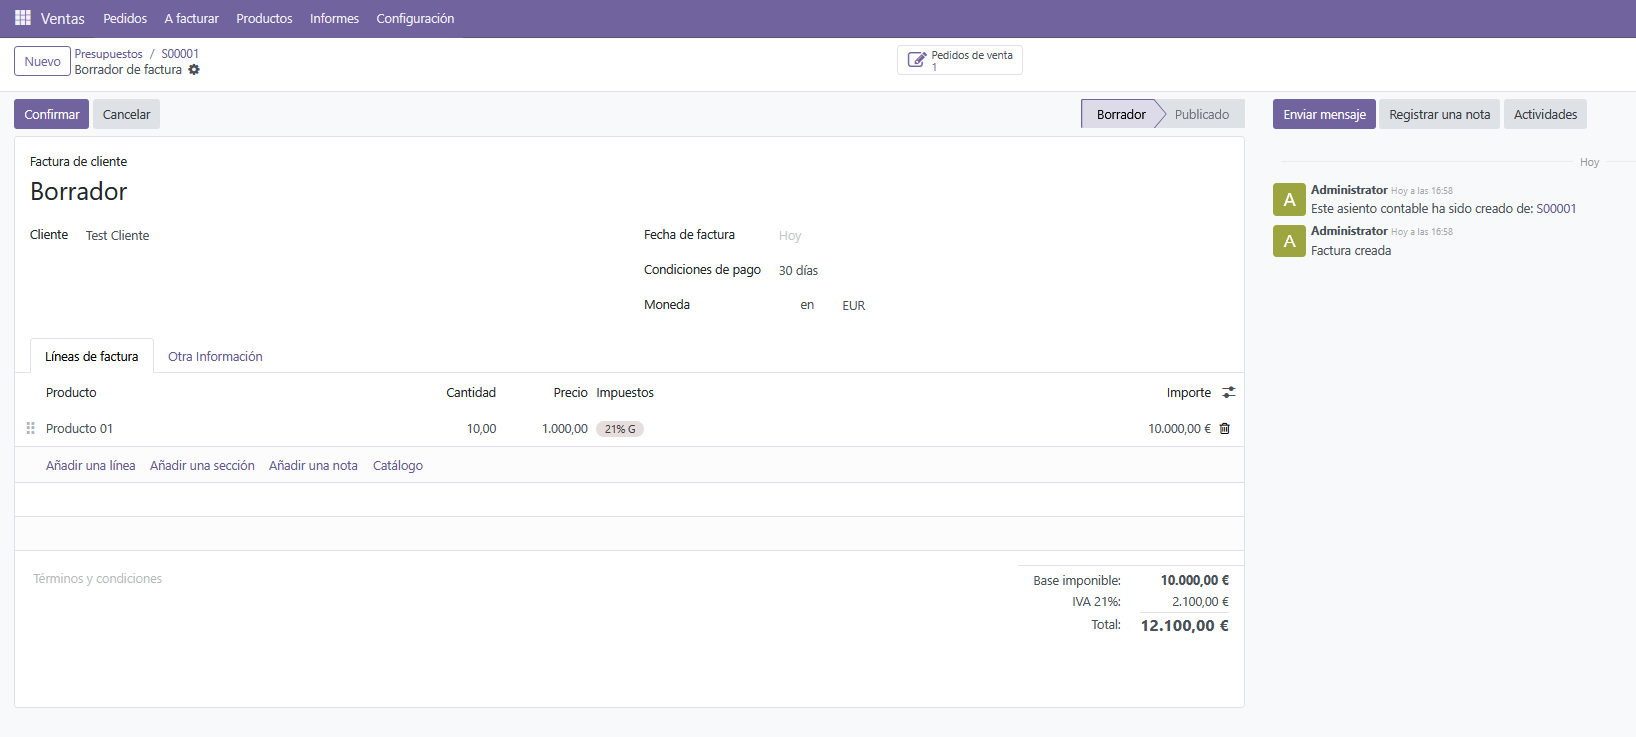
\includegraphics[width=1\textwidth]{pr2odoo45-borradorCreado.png}
    \caption{Borrador de factura creado}
\end{figure}
\FloatBarrier

\begin{figure}[h!]
    \centering
    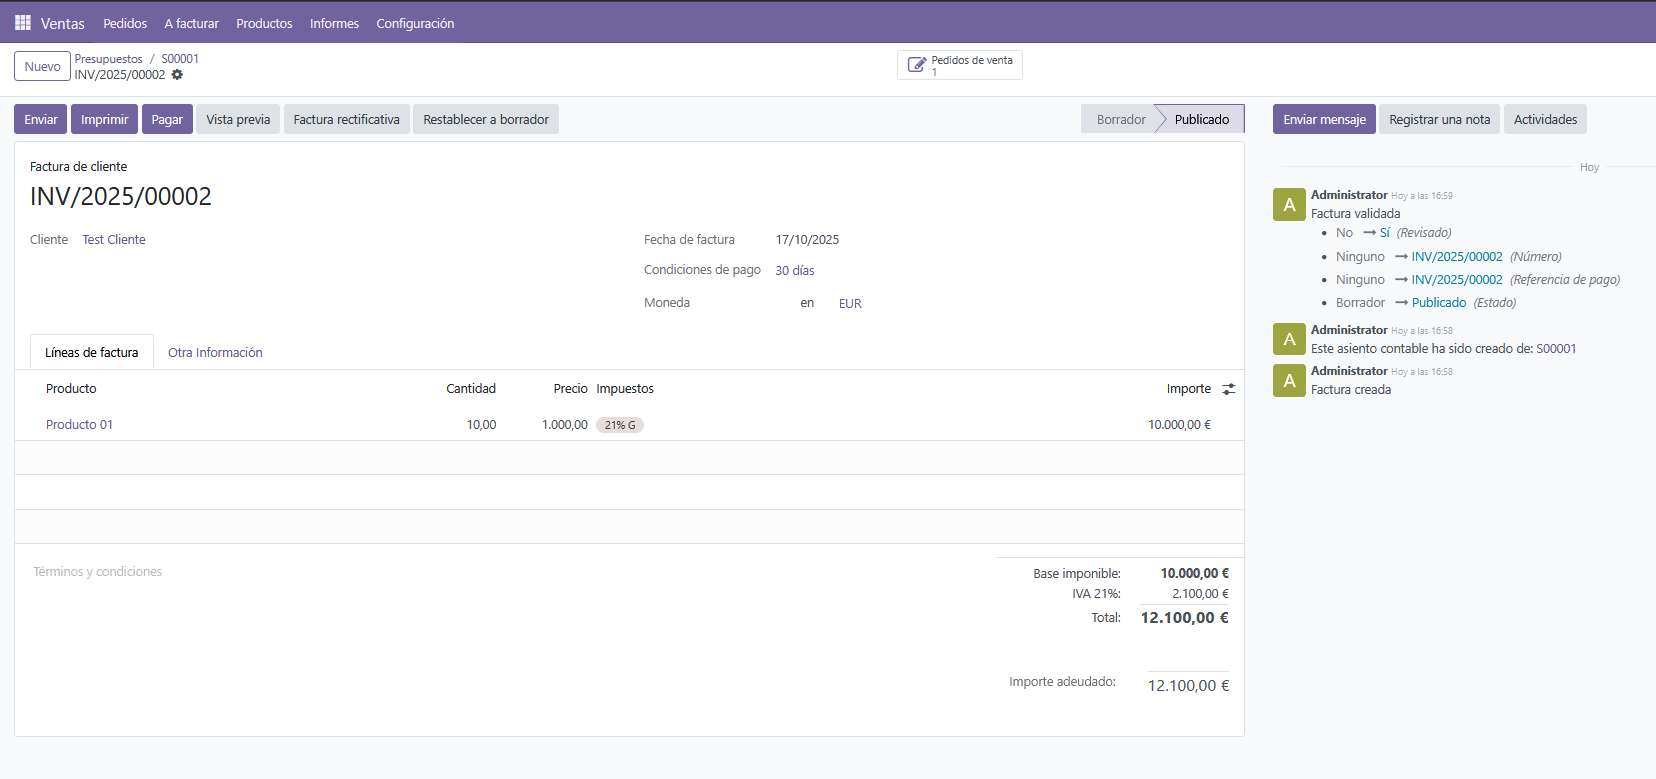
\includegraphics[width=1\textwidth]{pr2odoo46-facturaCreada.png}
    \caption{Factura creada}
\end{figure}
\FloatBarrier

\begin{figure}[h!]
    \centering
    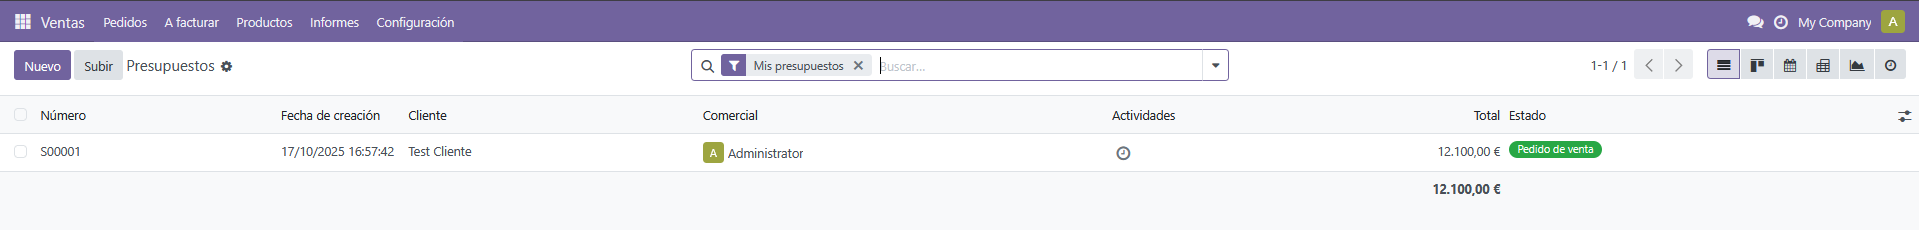
\includegraphics[width=1\textwidth]{pr2odoo47-listaVentas.png}
    \caption{Lista de ventas}
\end{figure}
\FloatBarrier

\clearpage

La pestaña de Pedidos se ocupa de:
\begin{itemize}
    \item Presupuestos
    \item Equipos de ventas
    \item Pedidos
    \item Clientes
\end{itemize}

La pestaña de A facturar se ocupa de pedidos a facturar y pedidos para ventas adicionales.

Productos lleva a su propia sección.

La pestaña de Informes se ocupa de:
\begin{itemize}
    \item Ventas
    \item Comerciales
    \item Productos
    \item Clientes
\end{itemize}

Las pestañas de configuración permiten:
\begin{itemize}
    \item Equipos de ventas
    \item Formato de pedidos
    \item Productos
    \item Pagos en línea
    \item Actividades
\end{itemize}

\clearpage

\subsection{Punto de venta}
\hyperlink{anchor-indice}{\textbf{Volver}}\\

El módulo de Punto de Venta permite para gestionar operaciones comerciales en tiempo real, incluso cuando no hay conexión a internet.

Puede realizar ventas rápidas y eficientes, gestionar efectivo y tarjetas, y mantener un control preciso de la caja registradora con una interfaz gráfica sencilla e intuitiva.

Una característica destacada es su capacidad para implementar programas de fidelidad y aplicar automáticamente descuentos o promociones a clientes frecuentes, mejorando así la experiencia del cliente y fomentando la lealtad hacia la marca.

\begin{figure}[h!]
    \centering
    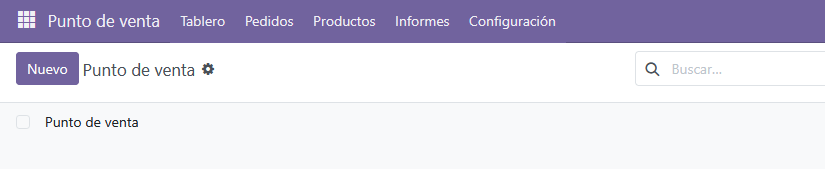
\includegraphics[width=1\textwidth]{pr2odoo48-pantallaPrincipal.png}
    \caption{Pantalla principal}
\end{figure}
\FloatBarrier

\begin{figure}[h!]
    \centering
    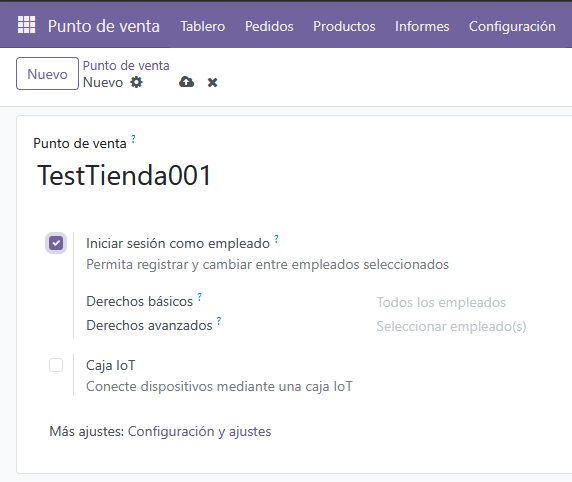
\includegraphics[width=1\textwidth]{pr2odoo49-nuevoTPV.png}
    \caption{Creación de punto de venta}
\end{figure}
\FloatBarrier

\begin{figure}[h!]
    \centering
    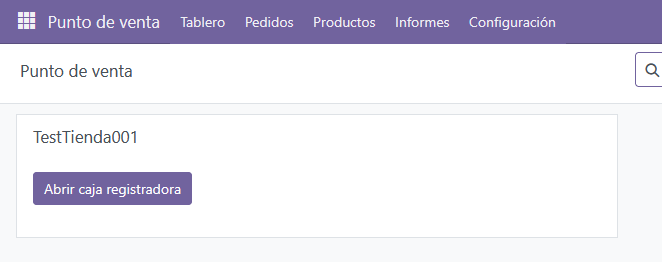
\includegraphics[width=1\textwidth]{pr2odoo50-tpvCreado.png}
    \caption{Punto de venta creado}
\end{figure}
\FloatBarrier

\begin{figure}[h!]
    \centering
    \includegraphics[width=1\textwidth]{pr2odoo51-modoAcceso.png}
    \caption{Modo de acceso (Usuario/PIN)}
\end{figure}
\FloatBarrier

\begin{figure}[h!]
    \centering
    \includegraphics[width=1\textwidth]{pr2odoo52-escojerCajero.png}
    \caption{Pantalla de seleccion de usuario}
\end{figure}
\FloatBarrier

\begin{figure}[h!]
    \centering
    \includegraphics[width=1\textwidth]{pr2odoo53-controlAperturaCaja.png}
    \caption{Pantalla de control de apertura de caja}
\end{figure}
\FloatBarrier

\begin{figure}[h!]
    \centering
    \includegraphics[width=1\textwidth]{pr2odoo54-creacionCliente.png}
    \caption{Creacion de nuevo cliente}
\end{figure}
\FloatBarrier

\begin{figure}[h!]
    \centering
    \includegraphics[width=1\textwidth]{pr2odoo55-clienteCreado.png}
    \caption{Cliente creado}
\end{figure}
\FloatBarrier

\begin{figure}[h!]
    \centering
    \includegraphics[width=1\textwidth]{pr2odoo56-operacionesCliente101.png}
    \caption{Operaciones con el cliente}
\end{figure}
\FloatBarrier

\begin{figure}[h!]
    \centering
    \includegraphics[width=1\textwidth]{pr2odoo57-diferentesClientesSimultaneos.png}
    \caption{Multiples clientes simultaneos}
\end{figure}
\FloatBarrier

\begin{figure}[h!]
    \centering
    \includegraphics[width=1\textwidth]{pr2odoo58-validacionPago.png}
    \caption{Validacion de pago}
\end{figure}
\FloatBarrier

\begin{figure}[h!]
    \centering
    \includegraphics[width=1\textwidth]{pr2odoo59-pagoCompletado101.png}
    \caption{Pago completado}
\end{figure}
\FloatBarrier

\begin{figure}[h!]
    \centering
    \includegraphics[width=1\textwidth]{pr2odoo60-cierreCaja.png}
    \caption{Cierre de caja}
\end{figure}
\FloatBarrier

\begin{figure}[h!]
    \centering
    \includegraphics[width=1\textwidth]{pr2odoo61-estadoFinalSesion.png}
    \caption{Estado final de sesión}
\end{figure}
\FloatBarrier

Cabe destacar que para crear categorias de productos, se puede crear desde el menu de Puntos de venta, y desde la pestaña "Puntos de Venta" de cada producto, asignarle la categoria que le corresponda.
\clearpage
Las pestañas de configuración permiten:
\begin{itemize}
    \item Tablero - Ver todas las tiendas creadas.
    \item Pedidos:
    \begin{itemize}
        \item  Pedidos.
        \item  Sesiones.
        \item  Pagos.
        \item  Clientes.
    \end{itemize}
    \item Productos - variantes y combinaciones.
    \item Informes de ventas, pedidos y de sesión.
    \item Configuración:
    \begin{itemize}
        \item  Ajustes de pago.
        \item  Terminal TPV.
        \item  Categorías de producto y atributos.
    \end{itemize}
\end{itemize}

\clearpage

\subsection{Contactos}
\hyperlink{anchor-indice}{\textbf{Volver}}\\

El módulo de Contactos funciona como el repositorio central de información sobre clientes, proveedores y socios comerciales.

Permite mantener un registro detallado y actualizado de toda la información relevante, incluyendo historial de interacciones, preferencias y datos demográficos.

Su integración con otros módulos permite sincronizar automáticamente la información y mantener una visión unificada de cada contacto a través de toda la organización, facilitando así la comunicación y la gestión de personal.

\begin{figure}[h!]
    \centering
    \includegraphics[width=1\textwidth]{pr2odoo62-pantallaPrincipal.png}
    \caption{Pantalla principal}
\end{figure}
\FloatBarrier

\begin{figure}[h!]
    \centering
    \includegraphics[width=1\textwidth]{pr2odoo63-edicionContacto.png}
    \caption{Edición de contacto}
\end{figure}
\FloatBarrier


\begin{figure}[h!]
    \centering
    \includegraphics[width=1\textwidth]{pr2odoo64-nuevoContacto.png}
    \caption{Nuevo contacto}
\end{figure}
\FloatBarrier


\begin{figure}[h!]
    \centering
    \includegraphics[width=1\textwidth]{pr2odoo65-opcionesContacto.png}
    \caption{Opciones de contacto}
\end{figure}
\FloatBarrier

Las pestañas de configuración permiten configurar:
\begin{itemize}
    \item Etiquetas y títulos de contacto
    \item Sectores
    \item Opciones de localización
    \item Datos de cuentas bancarias
\end{itemize}

\clearpage

\subsection{CRM}
\hyperlink{anchor-indice}{\textbf{Volver}}\\

El módulo CRM (Customer Relationship Management) permite enfocarse en los clientes y las necesidades de ventas, mediante seguimiento de leads y pronósticos precisos con el objetivo de cerrar oportunidades.

Cada oportunidad aparece en un entorno Kanban como una tarjeta en una lista con toda la información relevante y cada etapa muestra un resumen general de los ingresos esperados.

Este entorno Kanban permite organizar las oportunidades y moverlas según sea preciso.

\begin{figure}[h!]
    \centering
    \includegraphics[width=1\textwidth]{pr2odoo66-pantallaPrincipal.png}
    \caption{Pantalla principal}
\end{figure}
\FloatBarrier

\begin{figure}[h!]
    \centering
    \includegraphics[width=1\textwidth]{pr2odoo67-nuevaOportunidad.png}
    \caption{Nueva oportunidad}
\end{figure}
\FloatBarrier

\begin{figure}[h!]
    \centering
    \includegraphics[width=1\textwidth]{pr2odoo68-oportunidadCreada.png}
    \caption{Oportunidad creada}
\end{figure}
\FloatBarrier

\begin{figure}[h!]
    \centering
    \includegraphics[width=1\textwidth]{pr2odoo69-oportunidadOpciones.png}
    \caption{Opciones de oportunidad}
\end{figure}
\FloatBarrier

\begin{figure}[h!]
    \centering
    \includegraphics[width=1\textwidth]{pr2odoo70-oportunidadGanado.png}
    \caption{Cambio de estado: Ganado}
\end{figure}
\FloatBarrier

\begin{figure}[h!]
    \centering
    \includegraphics[width=1\textwidth]{pr2odoo71-oportunidadPerdida.png}
    \caption{Cambio de estado: Pantalla de Perdido}
\end{figure}
\FloatBarrier

\begin{figure}[h!]
    \centering
    \includegraphics[width=1\textwidth]{pr2odoo72-cambioDeEtapa.png}
    \caption{}
\end{figure}
\FloatBarrier

\begin{figure}[h!]
    \centering
    \includegraphics[width=1\textwidth]{pr2odoo72-cambioDeEtapa.png}
    \caption{Cambio de etapa desde interfaz de opciones}
\end{figure}
\FloatBarrier

\begin{figure}[h!]
    \centering
    \includegraphics[width=1\textwidth]{pr2odoo73-añadirOportunidadDirectamenteEnEtapa.png}
    \caption{Creacion de oportunidad directamente en la etapa deseada}
\end{figure}
\FloatBarrier

\begin{figure}[h!]
    \centering
    \includegraphics[width=1\textwidth]{pr2odoo74-crearEtapa.png}
    \caption{Creación de etapa}
\end{figure}
\FloatBarrier

\begin{figure}[h!]
    \centering
    \includegraphics[width=1\textwidth]{pr2odoo75-cambioManualDeEtapa.png}
    \caption{Cambio manual de etapa (en este caso, a Ganado)}
\end{figure}
\FloatBarrier

En la pestaña de Ventas se puede no solo ver el flujo actual, sino también generar nuevas actividades, ver y editar presupuestos, equipos y clientes.

Informes abarca las secciones de pronóstico, flujo, leads y actividades.

Configuración permite editar:
\begin{itemize}
    \item Equipos de ventas
    \item Actividades:
    \begin{itemize}
        \item Tipos.
        \item Planes.
    \end{itemize}
    \item Flujo:
    \begin{itemize}
        \item Etiquetas
        \item Razones de pérdida
    \end{itemize}
    \item Generación de leads: Solicitudes de minería.
\end{itemize}

\clearpage

\section{Copias de seguridad}
\hyperlink{anchor-indice}{\textbf{Volver}}\\

\subsection{Base de datos}

\subsubsection{Interfaz}

Dirección en navegador para realizar backup:
\begin{verbatim}
    http://localhost:9001/web/database/manager
\end{verbatim}


\begin{figure}[h!]
    \centering
    \includegraphics[width=1\textwidth]{pr2odoo76-backupInterfazPrincipal.png}
    \caption{Pantalla principal}
\end{figure}
\FloatBarrier

\begin{figure}[h!]
    \centering
    \includegraphics[width=1\textwidth]{pr2odoo77-backupInterfazPantallaCambio.png}
    \caption{Pantalla de backup}
\end{figure}
\FloatBarrier

\begin{figure}[h!]
    \centering
    \includegraphics[width=1\textwidth]{pr2odoo78-backupInterfazDescargado.png}
    \caption{Backup descargado}
\end{figure}
\FloatBarrier

\subsubsection{Comandos}
\hyperlink{anchor-indice}{\textbf{Volver}}\\

Comando: 
\begin{verbatim}
    docker ps
\end{verbatim}

\begin{figure}[h!]
    \centering
    \includegraphics[width=1\textwidth]{pr2odoo79-dockerPS.png}
    \caption{Información de los contenedores}
\end{figure}
\FloatBarrier

Comando: 
\begin{verbatim}
    docker exec 98832932c559 pg_dump -U odoo -F c odoo_test > C:\odoo_backups\odoo_backup.sql 
\end{verbatim}

\begin{itemize}
    \item 98832932c559: ID del contenedor
    \item odoo\_test: nombre de la base de datos
    \item C:/odoo\_backups/odoo\_backup.sql: ruta donde guardaremos la copia de seguridad
\end{itemize}

\begin{figure}[h!]
    \centering
    \includegraphics[width=1\textwidth]{pr2odoo80-comandoBackup.png}
    \caption{Comando para realizar backup}
\end{figure}
\FloatBarrier

\begin{figure}[h!]
    \centering
    \includegraphics[width=1\textwidth]{pr2odoo81-backupRealizado.png}
    \caption{Backup realizado}
\end{figure}
\FloatBarrier

\subsection{Archivo de configuración de Odoo}
\hyperlink{anchor-indice}{\textbf{Volver}}\\

Comando: 
\begin{verbatim}
    docker exec -it e0.bigodoo.net mkdir -p /etc/odoo
\end{verbatim}

\begin{itemize}
    \item e0.bigodoo.net: nombre del contenedor (el ID también es válido)
    \item /etc/odoo: directorio a crear
\end{itemize}

\begin{figure}[h!]
    \centering
    \includegraphics[width=1\textwidth]{pr2odoo82-crearDirectorio.png}
    \caption{Crear directorio de archivo de configuración}
\end{figure}
\FloatBarrier

Comando: 
\begin{verbatim}
    docker exec -it e0.bigodoo.net cp /etc/odoo/odoo.conf /etc/odoo/odoo.conf.backup
\end{verbatim}

\begin{itemize}
    \item e0.bigodoo.net: nombre del contenedor (el ID también es válido)
    \item /etc/odoo/odoo.conf: archivo a copiar
    \item /etc/odoo/odoo.conf.backup: ruta para la copia
\end{itemize}

\begin{figure}[h!]
    \centering
    \includegraphics[width=1\textwidth]{pr2odoo83-crearBackup.png}
    \caption{Crear archivo de backup}
\end{figure}
\FloatBarrier

Comando: 
\begin{verbatim}
    docker exec -it e0.bigodoo.net ls -la /etc/odoo/odoo.conf.backup
\end{verbatim}

\begin{itemize}
    \item e0.bigodoo.net: nombre del contenedor (el ID también es válido)
    \item /etc/odoo/odoo.conf.backup: archivo a comprobar
\end{itemize}

\begin{figure}[h!]
    \centering
    \includegraphics[width=1\textwidth]{pr2odoo84-comprobarBackup.png}
    \caption{Comprobar existencia de backup}
\end{figure}
\FloatBarrier

\clearpage

Comando: 
\begin{verbatim}
    docker cp e0.bigodoo.net:/etc/odoo/odoo.conf.backup C:/odoobackup
\end{verbatim}

\begin{itemize}
    \item e0.bigodoo.net: nombre del contenedor (el ID también es válido)
    \item /etc/odoo/odoo.conf.backup: archivo a copiar
    \item /etc/odoo/odoo.conf.backup: ruta para la copia en host
\end{itemize}

\begin{figure}[h!]
    \centering
    \includegraphics[width=1\textwidth]{pr2odoo85-copiarBackupAhost.png}
    \caption{Copiar archivo de backup a host}
\end{figure}
\FloatBarrier

\begin{figure}[h!]
    \centering
    \includegraphics[width=1\textwidth]{pr2odoo86-backupCopiado.png}
    \caption{Backup copiado a host}
\end{figure}
\FloatBarrier
\end{document}
